% =============================================================================
%  FAccT 2026 submission.
%
%  Format follows the ACM FAccT 2026 Author Guide: the ACM `acmart' class in
%  manuscript/screen/review/anonymous mode, up to 14 content pages including
%  figures and tables, unlimited references, one additional endmatter page, and
%  appendices that do not count toward the limit.
%
%  Line numbers are suppressed on purpose (\@ACM@reviewfalse below): the class
%  option string the Author Guide prescribes is kept verbatim, and only the
%  line-numbering side effect is turned off.
%
%  Numbers are NEVER hand-typed. Every quantity is either (a) a generated macro
%  \input from ../unified-report/generated/, (b) a generated tabular \input from
%  the same directory, or (c) plotted by figures/make_facct_figures.py, which
%  PARSES those same committed artifacts. See Appendix D.
% =============================================================================
\documentclass[manuscript,screen,review,anonymous]{acmart}

\setcopyright{none}
\settopmatter{printfolios=true,printccs=false,printacmref=false}
\renewcommand\footnotetextcopyrightpermission[1]{}
\pagestyle{plain}

\usepackage{booktabs}
\usepackage{multirow}
\usepackage{array}
\usepackage{float}
\usepackage{graphicx}
\usepackage{amsmath}
\usepackage{enumitem}
\usepackage{xcolor}
\usepackage{colortbl}
\usepackage[most]{tcolorbox}
\usepackage{tikz}
\usetikzlibrary{arrows.meta,positioning,shapes.geometric,fit,matrix}
\usepackage{microtype}
\usepackage[nameinlink,capitalize]{cleveref}

\graphicspath{{figures/}{../unified-report/figures/}}

% ---- palette, shared with figures/make_facct_figures.py ----------------------
\definecolor{bgblue}{HTML}{EAF2FF}
\definecolor{bgblueedge}{HTML}{2563EB}
\definecolor{tkgreen}{HTML}{EAF7EE}
\definecolor{tkgreenedge}{HTML}{15803D}
\definecolor{amberfill}{HTML}{FEF3C7}
\definecolor{amberedge}{HTML}{D97706}
\definecolor{cardgrey}{HTML}{F3F4F6}
\definecolor{inkgrey}{HTML}{374151}
\definecolor{guidealt}{HTML}{F5F7F9}

\newcommand{\code}[1]{\texttt{\small #1}}
\newcommand{\cmark}{\textcolor{tkgreenedge}{\ensuremath{\checkmark}}}
\newcommand{\xmark}{\textcolor{black!45}{\ensuremath{\times}}}

\newtcolorbox{background}[1]{colback=bgblue,colframe=bgblueedge,title={#1},
  fonttitle=\bfseries\small,fontupper=\small,boxrule=0.5pt,
  left=4pt,right=4pt,top=3pt,bottom=3pt,breakable}
\newtcolorbox{takeaway}[1]{colback=tkgreen,colframe=tkgreenedge,title={#1},
  fonttitle=\bfseries\small,fontupper=\small,boxrule=0.5pt,
  left=4pt,right=4pt,top=3pt,bottom=3pt,breakable}
\newtcolorbox{casebox}[1]{colback=amberfill!35,colframe=amberedge,title={#1},
  fonttitle=\bfseries\small,fontupper=\small,boxrule=0.6pt,arc=2pt,
  left=5pt,right=5pt,top=3pt,bottom=3pt}

% ---- generated macros: every number below is bound to a committed artifact ---
% Auto-generated by analyze_paper_a_sft.py -- do not edit by hand.
\newcommand{\RepDelta}{+0.3234}
\newcommand{\RepCILower}{+0.2647}
\newcommand{\RepCIUpper}{+0.3690}
\newcommand{\RepLCB}{+0.2725}
\newcommand{\TransferDelta}{-0.0589}
\newcommand{\TransferCILower}{-0.0837}
\newcommand{\TransferCIUpper}{-0.0321}
\newcommand{\TransferUCB}{-0.0362}
\newcommand{\TotalSeedCount}{20}
\newcommand{\SpecializationSeedCount}{15}
\newcommand{\UniformGainSeedCount}{5}
\newcommand{\UniformLossSeedCount}{0}
\newcommand{\TransferFavoredSeedCount}{0}
\newcommand{\ZeroAxisSeedCount}{0}
\newcommand{\RepBaseTPR}{0.1296}
\newcommand{\RepSFTTPR}{0.7686}
\newcommand{\RepDeltaTPR}{+0.6390}
\newcommand{\RepBaseTPRPct}{13.0}
\newcommand{\RepSFTTPRPct}{76.9}
\newcommand{\RepDeltaTPRPct}{+63.9}
\newcommand{\RepBaseFPR}{0.0169}
\newcommand{\RepSFTFPR}{0.0108}
\newcommand{\RepDeltaFPR}{-0.0061}
\newcommand{\RepBaseFPRPct}{1.7}
\newcommand{\RepSFTFPRPct}{1.1}
\newcommand{\RepDeltaFPRPct}{-0.6}
\newcommand{\RepBasePooledFPR}{0.0213}
\newcommand{\RepSFTPooledFPR}{0.0194}
\newcommand{\RepDeltaPooledFPR}{-0.0019}
\newcommand{\RepBasePooledFPRPct}{2.1}
\newcommand{\RepSFTPooledFPRPct}{1.9}
\newcommand{\RepDeltaPooledFPRPct}{-0.2}
\newcommand{\RepPositiveN}{313}
\newcommand{\RepNegativeN}{364}
\newcommand{\TransferBaseTPR}{0.5171}
\newcommand{\TransferSFTTPR}{0.5807}
\newcommand{\TransferDeltaTPR}{+0.0636}
\newcommand{\TransferBaseTPRPct}{51.7}
\newcommand{\TransferSFTTPRPct}{58.1}
\newcommand{\TransferDeltaTPRPct}{+6.4}
\newcommand{\TransferBaseFPR}{0.0805}
\newcommand{\TransferSFTFPR}{0.1546}
\newcommand{\TransferDeltaFPR}{+0.0741}
\newcommand{\TransferBaseFPRPct}{8.1}
\newcommand{\TransferSFTFPRPct}{15.5}
\newcommand{\TransferDeltaFPRPct}{+7.4}
\newcommand{\TransferBasePooledFPR}{0.0430}
\newcommand{\TransferSFTPooledFPR}{0.1704}
\newcommand{\TransferDeltaPooledFPR}{+0.1273}
\newcommand{\TransferBasePooledFPRPct}{4.3}
\newcommand{\TransferSFTPooledFPRPct}{17.0}
\newcommand{\TransferDeltaPooledFPRPct}{+12.7}
\newcommand{\TransferPositiveN}{790}
\newcommand{\TransferNegativeN}{790}
\newcommand{\ORBenchBaseFPR}{0.1181}
\newcommand{\ORBenchSFTFPR}{0.1201}
\newcommand{\ORBenchDeltaFPR}{+0.0020}
\newcommand{\ORBenchBaseFPRPct}{11.8}
\newcommand{\ORBenchSFTFPRPct}{12.0}
\newcommand{\ORBenchDeltaFPRPct}{+0.2}
\newcommand{\ORBenchN}{400}
\newcommand{\HarmBenchBaseRecall}{0.7800}
\newcommand{\HarmBenchSFTRecall}{0.6003}
\newcommand{\HarmBenchDeltaRecall}{-0.1797}
\newcommand{\HarmBenchBaseRecallPct}{78.0}
\newcommand{\HarmBenchSFTRecallPct}{60.0}
\newcommand{\HarmBenchDeltaRecallPct}{-18.0}
\newcommand{\HarmBenchN}{200}
   % \Rep*, \Transfer*, \HarmBench*, \ORBench*
% GENERATED by reproduce.py (matched_fpr.py) from artifacts/paper_a_sft_v2/scores/scores.parquet
\newcommand{\MatchedTransferBase}{0.517}
\newcommand{\MatchedTransferSft}{0.185}
\newcommand{\MatchedTransferDelta}{-0.332}
\newcommand{\MatchedHarmBase}{0.780}
\newcommand{\MatchedHarmSft}{0.171}
\newcommand{\MatchedHarmDelta}{-0.609}
\newcommand{\MatchedWorseTransfer}{4}
\newcommand{\MatchedWorseHarm}{4}
   % \Matched*
% GENERATED by reproduce.py (low_fpr.py) -- do not hand-edit.
\newcommand{\LowFprBudget}{0.05}
\newcommand{\LowFprChance}{0.025}
\newcommand{\LowFprNBoot}{2,000}
\newcommand{\LowFprRepApDelta}{+0.323}
\newcommand{\LowFprRepApBase}{0.658}
\newcommand{\LowFprRepApSft}{0.982}
\newcommand{\LowFprRepPAucDelta}{+0.686}
\newcommand{\LowFprRepPAucBase}{0.162}
\newcommand{\LowFprRepPAucSft}{0.848}
\newcommand{\LowFprRepTprDelta}{+0.678}
\newcommand{\LowFprRepTprBase}{0.254}
\newcommand{\LowFprRepTprSft}{0.932}
\newcommand{\LowFprRepAmplification}{2.1}
\newcommand{\LowFprTransApDelta}{-0.059}
\newcommand{\LowFprTransApBase}{0.866}
\newcommand{\LowFprTransApSft}{0.807}
\newcommand{\LowFprTransPAucDelta}{-0.174}
\newcommand{\LowFprTransPAucBase}{0.429}
\newcommand{\LowFprTransPAucSft}{0.255}
\newcommand{\LowFprTransTprDelta}{-0.199}
\newcommand{\LowFprTransTprBase}{0.558}
\newcommand{\LowFprTransTprSft}{0.360}
\newcommand{\LowFprTransAmplification}{3.0}
\newcommand{\LowFprWorstName}{Qwen3-4B}
\newcommand{\LowFprWorstAp}{-0.150}
\newcommand{\LowFprWorstPAuc}{-0.409}
\newcommand{\LowFprWorstPAucCI}{[-0.499, -0.312]}
\newcommand{\LowFprWorstTpr}{-0.437}
\newcommand{\LowFprSignFlips}{0}
        % \LowFpr*
% GENERATED by reproduce.py (low_fpr.py) -- do not hand-edit.
\newcommand{\LowFprKlBeta}{0.5}
\newcommand{\LowFprKlRepApDelta}{-0.035}
\newcommand{\LowFprKlRepPAucDelta}{-0.214}
\newcommand{\LowFprKlRepTprDelta}{-0.123}
\newcommand{\LowFprKlRepAmplification}{6.2}
\newcommand{\LowFprKlTransApDelta}{+0.061}
\newcommand{\LowFprKlTransPAucDelta}{+0.149}
\newcommand{\LowFprKlTransTprDelta}{+0.163}
\newcommand{\LowFprKlTransAmplification}{2.4}
\newcommand{\LowFprKlMarginMultipleAp}{1.7}
\newcommand{\LowFprKlMarginMultiplePAuc}{10.7}
     % \LowFprKl*
\input{../unified-report/generated/klsft_macros}         % \KL*
% AUTO-GENERATED by experiments/emit_adaptation_tex.py -- do not hand-edit.
\newcommand{\AdaNCheckpoints}{10}
\newcommand{\AdaNFamilies}{6}
\newcommand{\AdaNCheckpointsPB}{6}
\newcommand{\AdaNCheckpointsGen}{4}
\newcommand{\AdaNFamiliesPB}{5}
\newcommand{\AdaNFamiliesGen}{2}
\newcommand{\AdaNEvalFamilies}{2,140}
\newcommand{\AdaPrimaryBeta}{0.5}
\newcommand{\AdaMargin}{0.02}
\newcommand{\AdaHGain}{$+0.111$}
\newcommand{\AdaHGainLCB}{$+0.070$}
\newcommand{\AdaHConc}{$+0.183$}
\newcommand{\AdaHConcLCB}{$+0.137$}
\newcommand{\AdaHPreserve}{$+0.047$}
\newcommand{\AdaHPreserveLCB}{$+0.032$}
\newcommand{\AdaHCost}{$-0.034$}
\newcommand{\AdaHCostLCB}{$-0.062$}
\newcommand{\AdaHheldSFT}{$-0.072$}
\newcommand{\AdaRQoneCriterionMet}{true}
\newcommand{\AdaRQtwoCriterionMet}{false}
\newcommand{\AdaRQoneSupported}{true}
\newcommand{\AdaRQtwoSupported}{false}
\newcommand{\AdaMixedHGain}{$+0.174$}
\newcommand{\AdaMixedHGainLCB}{$+0.129$}
\newcommand{\AdaMixedHConc}{$+0.239$}
\newcommand{\AdaMixedHConcLCB}{$+0.189$}
\newcommand{\AdaMixedHPreserve}{$+0.049$}
\newcommand{\AdaMixedHCost}{$-0.036$}
\newcommand{\AdaGenHGain}{$+0.324$}
\newcommand{\AdaGenHConc}{$+0.373$}
\newcommand{\AdaGenHPreserve}{$+0.058$}
\newcommand{\AdaGenHCost}{$-0.036$}
\newcommand{\AdaNFamiliesPBValid}{4}
\newcommand{\AdaNullDilution}{$5/4 = 1.25\times$}
\newcommand{\AdaHGainDropNull}{$+0.139$}
\newcommand{\AdaHGainLCBDropNull}{$+0.088$}
\newcommand{\AdaHConcDropNull}{$+0.229$}
\newcommand{\AdaHConcLCBDropNull}{$+0.171$}
\newcommand{\AdaHPreserveDropNull}{$+0.059$}
\newcommand{\AdaHPreserveLCBDropNull}{$+0.040$}
\newcommand{\AdaHCostDropNull}{$-0.043$}
\newcommand{\AdaHCostLCBDropNull}{$-0.077$}
\newcommand{\AdaGammaGain}{$-0.213$}
\newcommand{\AdaGammaGainCI}{$[-0.240, -0.179]$}
\newcommand{\AdaGammaGainExcludesZero}{true}
\newcommand{\AdaGammaConc}{$-0.190$}
\newcommand{\AdaGammaConcCI}{$[-0.223, -0.151]$}
\newcommand{\AdaGammaConcExcludesZero}{true}
\newcommand{\AdaGammaPreserve}{$-0.011$}
\newcommand{\AdaGammaPreserveCI}{$[-0.031, +0.010]$}
\newcommand{\AdaGammaPreserveExcludesZero}{false}
\newcommand{\AdaGammaCost}{$+0.002$}
\newcommand{\AdaGammaCostCI}{$[-0.016, +0.019]$}
\newcommand{\AdaGammaCostExcludesZero}{false}
\newcommand{\AdaGammaHeldSFT}{$-0.023$}
\newcommand{\AdaGammaHeldSFTCI}{$[-0.042, -0.003]$}
\newcommand{\AdaGammaHeldSFTExcludesZero}{true}
    % \Ada*
% GENERATED by reproduce.py from artifacts/expguard_external/ (frontier.py)
\newcommand{\FrontierBestName}{gpt-5.4 (low)}
\newcommand{\FrontierBestTpr}{.896}
\newcommand{\FrontierBestAp}{.9773}
\newcommand{\FrontierBestBaseName}{SmolLM3-3B}
\newcommand{\FrontierBestBaseTpr}{.787}
\newcommand{\FrontierBestOpenName}{Qwen3-32B}
\newcommand{\FrontierBestOpenTpr}{.830}
\newcommand{\FrontierBestOpenParams}{32}
\newcommand{\FrontierBestSftName}{Qwen3-32B}
\newcommand{\FrontierBestSftTpr}{.809}
\newcommand{\FrontierNSeeds}{5}
\newcommand{\FrontierGainOverOpen}{+0.066}
\newcommand{\FrontierGainOverOpenCI}{[+0.043, +0.089]}
\newcommand{\FrontierGainOverBase}{+0.109}
\newcommand{\FrontierGainOverBaseCI}{[+0.077, +0.139]}
\newcommand{\FrontierScaleGain}{+0.062}
\newcommand{\FrontierScaleGainCI}{[+0.039, +0.084]}
\newcommand{\FrontierScaleFactor}{8}
\newcommand{\FrontierEightBvsFourB}{-0.020}
\newcommand{\FrontierEightBvsFourBCI}{[-0.050, +0.001]}
\newcommand{\FrontierSftMeanDelta}{+0.005}
\newcommand{\FrontierSftWorstName}{SmolLM3-3B}
\newcommand{\FrontierSftWorstDelta}{-0.059}
\newcommand{\FrontierSftBestName}{SmolLM2-1.7B}
\newcommand{\FrontierSftBestDelta}{+0.122}
\newcommand{\FrontierSftNumHurt}{4}
\newcommand{\FrontierSftNumTotal}{6}
\newcommand{\FrontierScaleTunedName}{Qwen3-32B}
\newcommand{\FrontierScaleTunedParams}{32}
\newcommand{\FrontierScaleTunedRepGain}{+0.037}
\newcommand{\FrontierScaleTunedTransferCost}{-0.117}
\newcommand{\FrontierScaleTunedRep}{.9903}
\newcommand{\FrontierScaleTunedTransfer}{.8447}
\newcommand{\FrontierScaleUntunedRep}{.9533}
\newcommand{\FrontierScaleUntunedTransfer}{.9620}
\newcommand{\FrontierScaleTunedExpguardDelta}{-0.020}
\newcommand{\FrontierBestMedianMs}{1,553}
\newcommand{\FrontierBestCost}{0.80}
\newcommand{\FrontierSlowdown}{77}
      % \Frontier*
% AUTO-GENERATED by experiments/emit_frontier_general_h2h_tex.py -- do not hand-edit.
\newcommand{\HtwoRef}{gpt-5.4 / low}
\newcommand{\HtwoBudget}{5\%}
\newcommand{\HtwoNRepSources}{3}
\newcommand{\HtwoNTransSources}{2}
\newcommand{\HtwoRepSources}{\code{jailbreak\_classification}, \code{prompt\_injections}, \code{toxicchat}}
\newcommand{\HtwoAggDeltaTpr}{$+0.083$}
\newcommand{\HtwoAggDeltaTprCI}{$[+0.013, +0.157]$}
\newcommand{\HtwoAggDeltaAp}{$+0.039$}
\newcommand{\HtwoAggDeltaApCI}{$[+0.015, +0.072]$}
\newcommand{\HtwoAggSignificant}{true}
\newcommand{\HtwoNCells}{12}
\newcommand{\HtwoNSigNominal}{3}
\newcommand{\HtwoNSigHolm}{0}
\newcommand{\HtwoBestName}{Qwen2.5-1.5B}
\newcommand{\HtwoBestSource}{\code{prompt\_injections}}
\newcommand{\HtwoBestN}{67}
\newcommand{\HtwoBestTpr}{.948}
\newcommand{\HtwoBestAuroc}{0.9928}
\newcommand{\HtwoRefTpr}{.741}
\newcommand{\HtwoRefAuroc}{0.8731}
\newcommand{\HtwoBestDeltaTpr}{$+0.207$}
\newcommand{\HtwoBestDeltaTprCI}{$[+0.042, +0.389]$}
\newcommand{\HtwoBestDeltaTprHolm}{$[-0.072, +0.486]$}
\newcommand{\HtwoBestHolmSig}{false}
\newcommand{\HtwoBestPBoot}{0.011}
\newcommand{\HtwoBestPHolm}{0.132}
\newcommand{\HtwoHolmFirstThreshold}{0.0042}
\newcommand{\HtwoMaxTCrit}{3.07}
\newcommand{\HtwoBestDeltaAp}{$+0.103$}
\newcommand{\HtwoBestDeltaApCI}{$[+0.032, +0.196]$}
\newcommand{\HtwoNBoot}{2,000}
\newcommand{\HtwoNSig}{3}
\newcommand{\HtwoNSftCells}{12}
\newcommand{\HtwoAggEqSourceTpr}{$+0.083$}
\newcommand{\HtwoAggEqSourceTprCI}{$[+0.013, +0.157]$}
\newcommand{\HtwoAggEqCellTpr}{$+0.083$}
\newcommand{\HtwoAggEqCellTprCI}{$[+0.013, +0.157]$}
\newcommand{\HtwoAggRowWTpr}{$+0.049$}
\newcommand{\HtwoAggRowWTprCI}{$[-0.031, +0.112]$}
\newcommand{\HtwoAggWithBaseTpr}{$-0.264$}
\newcommand{\HtwoAggWithBaseTprCI}{$[-0.321, -0.179]$}
\newcommand{\HtwoAggSrcResampledCI}{$[-0.019, +0.220]$}
\newcommand{\HtwoAggSrcResampledExcludesZero}{false}
\newcommand{\HtwoTransRefTpr}{.967}
\newcommand{\HtwoTransBestLocalName}{Qwen3-4B base}
\newcommand{\HtwoTransBestLocalTpr}{.917}
           % \Htwo*
% Generated by code/build_pilot_artifacts.py; do not edit by hand.
\newcommand{\PilotEvidenceStatus}{\texttt{clean\_v2\_retrospective\_estimation}}
\newcommand{\PilotNModels}{4}
\newcommand{\PilotNSeeds}{5}
\newcommand{\PilotNRepresentedBenchmarks}{3}
\newcommand{\PilotNTransferBenchmarks}{4}
\newcommand{\PilotNAPDatasets}{7}
\newcommand{\PilotNTransferPositiveVsBase}{2}
\newcommand{\PilotNSeedPairs}{10}
\newcommand{\PilotBaseRepresented}{0.658}
\newcommand{\PilotBaseTransfer}{0.866}
\newcommand{\PilotSFTRepresented}{0.982}
\newcommand{\PilotSFTTransfer}{0.807}
\newcommand{\PilotCompositionRepresented}{0.962}
\newcommand{\PilotCompositionTransfer}{0.883}
\newcommand{\PilotLogitTransfer}{0.891}
\newcommand{\PilotRepDeltaSFT}{-0.019}
\newcommand{\PilotRepDeltaSFTBootstrapMean}{-0.019}
\newcommand{\PilotRepDeltaSFTLow}{-0.031}
\newcommand{\PilotRepDeltaSFTHigh}{-0.010}
\newcommand{\PilotTransferDeltaSFT}{+0.076}
\newcommand{\PilotTransferDeltaSFTBootstrapMean}{+0.075}
\newcommand{\PilotTransferDeltaSFTLow}{+0.058}
\newcommand{\PilotTransferDeltaSFTHigh}{+0.093}
\newcommand{\PilotTransferDeltaBase}{+0.017}
\newcommand{\PilotTransferDeltaBaseBootstrapMean}{+0.017}
\newcommand{\PilotTransferDeltaBaseLow}{+0.005}
\newcommand{\PilotTransferDeltaBaseHigh}{+0.030}
\newcommand{\PilotTargetFPRPct}{5}
\newcommand{\PilotBaseTransferFPRPct}{8.1}
\newcommand{\PilotSFTTransferFPRPct}{15.5}
\newcommand{\PilotCompositionTransferFPRPct}{11.4}
\newcommand{\PilotConvexWeight}{0.95}
\newcommand{\PilotLockHashShort}{cabc8dee}
\newcommand{\PilotScoreHashShort}{b941ddba}
\newcommand{\PilotCompositionHashShort}{92c2cbc3}
         % \Pilot*
% GENERATED by mortgage-benchmark/tools/emit_composition_tex.py -- do not hand-edit.
\newcommand{\MortNRows}{994}
\newcommand{\MortNContentFamilies}{958}
\newcommand{\MortNContentFamiliesSpanning}{0}
\newcommand{\MortNProtectedPairs}{39}
\newcommand{\MortNProtectedPairsSpanning}{1}
\newcommand{\MortNProtectedPairsPublicOnly}{3}
\newcommand{\MortSpanningPairID}{PAIR-0000\#1}
\newcommand{\MortEmptyQuadrant}{G1/D0}
\newcommand{\MortNEmptyQuadrantRows}{0}
 % \Mort*
% GENERATED by reproduce.py -- coverage of the generated/ surface, do not hand-edit.
\newcommand{\ReproNInputs}{31}
\newcommand{\ReproNVerified}{16}
\newcommand{\ReproNEnvGated}{4}
\newcommand{\ReproNUncovered}{11}
\newcommand{\ReproNFailed}{0}
         % \Repro*
\input{../unified-report/generated/teaser_macros}        % \Teaser*

\title{Benchmark Gains Are Not Governance Gains}
\subtitle{Paired, Budget-Matched Evaluation of Small Safety Guards Under Domain Shift}

\author{}

\begin{document}

% Keep the Author Guide's class-option string verbatim while suppressing the
% line numbers it would otherwise switch on.
\makeatletter\@ACM@reviewfalse\makeatother

\begin{abstract}
A \emph{safety guard} --- a small classifier that labels an incoming request \code{safe} or \code{unsafe}
before a language-model system acts on it --- is the mechanism by which a written content policy becomes
an enforced decision. Guards are chosen by a rule that is itself never audited: fine-tune a small open
model on available moderation data, score it on a public suite, ship the best checkpoint. We treat that
rule as the object of study and ask what a benchmark gain is valid \emph{for}.

We evaluate four small open checkpoints ($4\times5$ seeds) under a protocol with four commitments: each
tuned guard is compared only with its \emph{own} pre-tuning checkpoint on identical rows; sources named
in the training manifest are separated from sources held out at the source level; recalls are read only
at \emph{matched false-alarm budgets}; and three tiers of evidence are never pooled. The headline changes
under each. Fine-tuning raises macro average precision on represented sources by \RepDelta{}
[\RepCILower, \RepCIUpper] while held-out transfer moves \TransferDelta{}
[\TransferCILower, \TransferCIUpper], pooling per-checkpoint effects of opposite sign. Read at each base
guard's own alarm rate, the apparent transfer-recall gain \emph{reverses} on all four checkpoints
(\MatchedTransferBase{}~$\rightarrow$~\MatchedTransferSft), and recall on hard attacks falls
\MatchedHarmBase{}~$\rightarrow$~\MatchedHarmSft. Restricted to the alarm budget an inline guard can
afford, the same comparison is $\LowFprTransAmplification\times$ larger; and the sourcing conclusion ---
self-host or buy a hosted frontier model --- \emph{inverts} between traffic a manifest represents and
traffic it does not.

A frozen, dual-labeled mortgage benchmark then isolates the stratum a general-safety score cannot see:
requests that read as ordinary professional prose while soliciting redlining by proxy or a pretextual
adverse-action reason. All four guards rank one such request \emph{below} the median benign inquiry in
the same split, and the protected-attribute invariance gate we built to check them fails its own
robustness test --- reported here as a negative result about instrument design. Our contribution is an
evidence discipline, not a new guard: four disclosures, computable from per-row scores an operator
already holds, that make specialization, threshold drift, and domain blindness legible before a
benchmark number is allowed to license a deployment claim.
\end{abstract}

\keywords{safety guards, content moderation, evaluation validity, distribution shift, algorithmic
auditing, fair lending, measurement}

\maketitle

% =============================================================================
\section{Introduction}
\label{sec:intro}

Between a user's request and a language-model system's response there is increasingly a second, much
smaller model whose only job is to decide whether the request may proceed. These \emph{guards} ---
Llama~Guard, WildGuard, ShieldGemma, Granite~Guardian, Qwen3Guard, and a long tail of in-house fine-tunes
\citep{inan2023llamaguard,han2024wildguard,zeng2024shieldgemma,padhi2024graniteguardian,qwen3guard2025}
--- are the point at which a written policy stops being a document and becomes an enforced decision about
a particular person's particular request. They are governance infrastructure in the sense
\citet{gorwa2020algorithmic} and \citet{gillespie2018custodians} describe for platform moderation: small,
cheap, invisible, and consequential.

How does an operator choose one? Overwhelmingly by a rule that is never itself audited: take a compact
instruction model, attach a low-rank adapter, fine-tune on whatever moderation data is at hand
\citep{elesedy2024loraguard,hu2021lora}, score the result on a public guardrail suite
\citep{bassani2024guardbench}, and keep the best-scoring checkpoint. The rule is cheap, reproducible,
and --- as an argument that the resulting system is fit to screen real traffic --- close to vacuous.

Our claim is not that fine-tuning harms guards. It is narrower: \textbf{a benchmark gain measures
something, and that something is usually not what the deployment decision needs to know.} Following the
measurement-modelling tradition in this venue
\citep{jacobs2021measurement,raji2021everything,blodgett2021salmon}, we ask what construct a guard score
operationalizes, and find four places where the operationalization and the deployment claim come apart.
Each is demonstrated on a fixed panel of four small open checkpoints, and each is a \emph{reporting}
failure before it is a modelling one:

\begin{enumerate}[leftmargin=1.6em,itemsep=1pt]
  \item \textbf{Whose sources?} The score rises sharply on the corpora the guard's own training manifest
  names and does not, on average, move on corpora held out at the source level: it measures acquaintance
  with the instrument, not the construct (\Cref{sec:finding-source}).
  \item \textbf{At whose alarm rate?} The apparent off-source recall gain is bought by alarming far more
  often; equalize the false-alarm budget and it reverses on every checkpoint, hardest on the hardest
  attacks, and restricting the metric to the region an inline guard operates in roughly triples the cost
  (\Cref{sec:finding-operational}).
  \item \textbf{On whose traffic?} Against a hosted frontier model on identical rows at a common budget,
  the small guards \emph{lose} on unfamiliar prompts and \emph{win} on sources their manifest names ---
  the ordering is a property of the traffic regime, not of the model, so one number cannot support a
  sourcing decision (\Cref{sec:finding-regime}).
  \item \textbf{Against whose policy?} In a regulated domain the dangerous request is often fluent,
  polite, procedurally framed text with no jailbreak, slur, or injection, for which a general-safety
  taxonomy has no label; we isolate that stratum with a dual-labeled, HMDA-grounded mortgage benchmark
  and show a worked miss (\Cref{sec:finding-construct}).
\end{enumerate}

\Cref{fig:findings} is those four findings in one spread. The distributive stakes deserve stating at
the outset, because the aggregates hide them: a guard's false positives fall on legitimate users whose
requests are blocked, its false negatives on whoever is harmed when a request is honored. On this panel
fine-tuning moves \emph{both} the wrong way off-source at once --- pooled false alarms on held-out
negatives climb $\TransferBasePooledFPRPct\%\!\rightarrow\!\TransferSFTPooledFPRPct\%$ while recall on
\code{HarmBench} attacks falls
$\HarmBenchBaseRecallPct\%\!\rightarrow\!\HarmBenchSFTRecallPct\%$. That is not a trade-off between two
populations but a loss for both, invisible to the represented-source number that would have justified
the deployment.

\begin{figure*}[t]
\centering
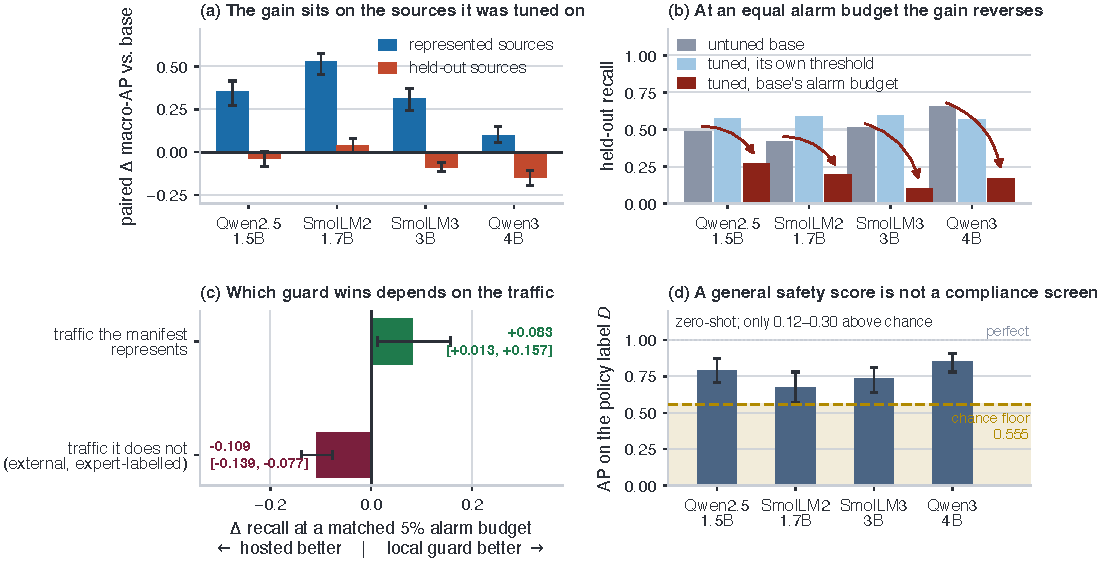
\includegraphics[width=\linewidth]{fig_facct_findings.pdf}
\caption{\textbf{Four ways a guard's benchmark score fails to answer the deployment question.}
\textbf{(a)} Paired change in macro average precision against each guard's \emph{own} pre-tuning
checkpoint on identical rows: large and uniform on the corpora the training manifest names, near zero
and split in sign on corpora held out at the source level. \textbf{(b)} Held-out recall at three
thresholds; the middle bar is the tuned guard at its own calibrated cutoff --- the comparison a
leaderboard reports --- where it alarms roughly four times as often on held-out negatives as its base.
\textbf{(c)} The same comparison against a hosted frontier reference at a matched $5\%$ budget points in
opposite directions on the two traffic regimes (upper bar: a post-hoc summary over \HtwoNRepSources{}
purposively chosen corpora; lower: a paired comparison on external expert-annotated rows).
\textbf{(d)} The same checkpoints, zero-shot, ranking a mortgage-policy violation label against the
chance floor its own prevalence sets. Every plotted value is parsed by
\code{figures/make\_facct\_figures.py} from the committed artifacts the tables
\code{\textbackslash input}, so no panel can drift from its table.}
\label{fig:findings}
\end{figure*}

\paragraph{Contributions.} (i) A \textbf{validity-first evaluation protocol} built from four commitments
--- strict pairing, source-level regime separation, matched alarm budgets, non-pooled evidence tiers ---
stated so a reader can check whether any published guard result satisfies them (\Cref{sec:protocol}).
(ii) The \textbf{demonstration that each commitment is load-bearing}: dropping any one changes the sign
or magnitude of the headline. (iii) A \textbf{dual-labeled regulated-domain instrument}, a worked
end-to-end miss, and an honest negative result about the protected-attribute gate we built alongside it
(\Cref{sec:finding-construct}). (iv) A \textbf{disclosure schedule} mapping each finding to the artifact
an auditor, procurement reviewer, or regulator needs to read a guard benchmark correctly
(\Cref{sec:governance}).

\paragraph{What we do not claim.} We introduce no model, metric, or training algorithm. The main
analysis is retrospective and estimation-only on a purposively chosen panel inspected during
development; intervals are conditional on that panel and are not hypothesis tests. The mortgage labels
are model-assigned against written policy cards, \emph{not} adjudicated by counsel or subject-matter
experts. Nothing here is a causal claim, a universal claim about fine-tuning, a deployment
recommendation, or a fair-lending finding (\Cref{sec:limitations}, \Cref{tab:ledger}).

% =============================================================================
\section{Guards as Governance Infrastructure}
\label{sec:background}

\subsection{The object, and the inference under audit}

The guards we study are prompt classifiers. Given a request $x$, a compact decoder-only model is prompted
with a fixed template and its verdict read as a single-token margin --- the difference of two decision
logits, one forward pass, no generation:
\begin{equation}
s(x) \;=\; z_{\text{unsafe}}(x) - z_{\text{safe}}(x) .
\label{eq:head}
\end{equation}
A threshold $\tau$ turns $s(x)$ into \code{block} or \code{allow}, and everything downstream of that
comparison --- who is refused service, which violating request proceeds --- is decided by the pair
$(s,\tau)$. The evaluation literature reports mostly $s$.

Two features of the setting are routinely elided. The errors are \emph{asymmetric in incidence}, not
merely in cost --- a false positive is borne by a user with a legitimate request, a false negative by
whoever the honored request harms --- so one accuracy number aggregates across populations with no
common welfare denominator, the objection \citet{selbst2019abstraction} raise to abstraction boundaries
drawn for modelling convenience. And a guard is a \emph{screening layer in front of a decision}, exactly
where \citet{raji2022fallacy} argue functionality rather than fairness is the first thing to interrogate:
a guard that does not work is not a fairness problem to mitigate but a non-functional component whose
deployment was licensed by a bad measurement.

The selection rule's implicit inference --- that a higher score is evidence of a better screening layer
--- must cross four gaps: from the benchmark's sources to real traffic; from a threshold-free ranking
metric to a specific operating point; from a balanced pool to a real prevalence of unsafe requests; and
from a general-safety taxonomy to the policy the operator must enforce. Each is known in isolation; what
is missing is a protocol that measures all four \emph{on the same rows for the same checkpoint}, so the
size of each gap can be set against the size of the reported gain. In \Citet{jacobs2021measurement}'s
terms these are four threats to the validity of one inference --- source, operational, regime, and
construct validity --- and
\Cref{sec:finding-source,sec:finding-operational,sec:finding-regime,sec:finding-construct} take them in
turn.

\subsection{Related work}
\label{sec:related}

Three strands meet here, and \Cref{app:related} discusses each at length.
\emph{Evaluation validity}: benchmarks under-determine the claims made from them --- general-capability
framings outrun what a fixed dataset supports \citep{raji2021everything}, fairness benchmarks carry
construct failures \citep{blodgett2021salmon}, behavioural testing beats aggregate scores
\citep{bowman2021benchmarking,ribeiro2020checklist}, progress on a fixed test set need not survive a
change of collection process \citep{recht2019imagenet,taori2020measuring}, and generative-AI evaluations
sit at a distance from the outcomes they are invoked to predict
\citep{weidinger2023sociotechnical,solaiman2023socialimpact,liao2023sociotechnicalgap}. Where model
cards and datasheets \citep{mitchell2019modelcards,gebru2021datasheets,hutchinson2021accountability}
established that documentation is part of the artifact, audit frameworks
\citep{raji2020closing,metaxa2021auditing,raji2022outsider} established who consumes it;
\Cref{sec:governance} is written in that idiom, and \citet{kapoor2023leakage} is our closest
methodological precedent for treating ``was the evaluation \emph{source} represented in training?'' as a
first-class reported quantity. \emph{Guard evaluation}: released guards
\citep{inan2023llamaguard,han2024wildguard,zeng2024shieldgemma,padhi2024graniteguardian,qwen3guard2025}
are typically reported against in- and out-of-distribution blocks, adapting a general model into a guard
is standard \citep{elesedy2024loraguard}, and adjacent work finds safety degradation tracking dataset
similarity \citep{hsiung2025guardrails}, policy overfitting \citep{liu2026domaingeneralizable}, surface
heuristics \citep{li2026surfaceheuristics}, evadability
\citep{hackett2025bypassing,bassani2025robustness}, poor calibration \citep{liu2025calibration}, and
domain fine-tuning of released guards \citep{hossain2026safetygeometry,lee2025saferoute,achara2025watchdogs}.
\emph{Policy-grounded and regulated-domain evaluation}: human-labelled policy-compliance benchmarks
\citep{cisnerosvelarde2026policy,choi2026compass}, regulation-grounded data
\citep{zhao2026mlbenchguard}, the canonical account of facially neutral proxies
\citep{barocas2016disparate}, its measurement in consumer lending \citep{bartlett2022fintech}, and
language models audited as underwriters \citep{bowen2024mortgage}; our protected-pair design is the
standard counterfactual token-fairness construction
\citep{kusner2017counterfactual,garg2019counterfactual}, repurposed from decision correctness to score
invariance. \Cref{tab:closest} places the closest work against the axes we measure: no row does all of
it, and almost every column has a row that does that column better than we do.

% =============================================================================
\section{The Protocol and Its Four Commitments}
\label{sec:protocol}

\paragraph{C1: compare a guard only with itself.} Leaderboard comparisons put model $X$'s guard beside
model $Y$'s, confounding ``the fine-tune helped'' with ``$X$ was a better starting point.'' We hold the
checkpoint fixed and compare every tuned guard with its \emph{own} pre-tuning weights, on identical
rows, through the identical head of \Cref{eq:head} and the identical tie-aware metric, reporting a
within-checkpoint change $\Delta = \mathrm{SFT}-\mathrm{base}$. This is the only construction that
attributes a movement to the intervention rather than to the luck of the starting point, and it is what
makes the sign splits in \Cref{fig:findings}(a) interpretable rather than noise.

\paragraph{C2: separate represented from source-held-out.} Every guard and its base are scored in two
disjoint regimes. \emph{Represented} rows are held back from the three corpora the manifest names
(\code{toxicchat} \citep{lin2023toxicchat}, \code{prompt\_injections},
\code{jailbreak\_classification}); \emph{transfer} rows come from four corpora whose \emph{sources} were
never trained on \citep{chao2024jailbreakbench,rottger2024xstest,han2024wildguard,jiang2024wildteaming};
and two single-class stress sets isolate the failure directions, \code{OR-Bench}
\citep{cui2024orbench} for over-refusal and \code{HarmBench} \citep{mazeika2024harmbench} for missed
catches. The row-level/source-level distinction is where guard papers most often equivocate: held-out
\emph{rows} from a represented corpus measure whether the guard learned that corpus's label conventions,
held-out \emph{sources} whether it learned anything portable, and reporting the first as generalization
is the leakage-shaped error \citet{kapoor2023leakage} catalogue, committed at corpus rather than row
level. We audit it --- a committed overlap audit finds no exact, normalized, $n$-gram-containment
($\geq0.80$), or character-shingle (Jaccard $\geq0.70$) overlap between manifest and transfer suite, and
no evaluation-family collisions --- while noting that the \emph{represented} splits are not clean in the
same sense ($1.6\%$--$5.0\%$ of each sits within Jaccard $0.70$ of a training row), which qualifies the
represented margins, not the transfer ones.

\paragraph{C3: read recalls only at matched alarm budgets.} A recall compared at unequal false-alarm
rates is not a comparison of discriminative power but of two different policies. We therefore report
thresholded quantities twice: at each guard's own calibration-selected cutoff, and with the tuned guard
re-thresholded so its pooled false-alarm rate on the evaluated negatives \emph{matches its own base's}.
Only the second licenses a sentence about catching more or less. One limit travels with every such
number: the budget is located by a quantile of the \emph{evaluated} negatives and recall measured on
those same rows, so it reads two ROC curves at a common point but is \emph{not} a threshold a
production system could place, since placing it requires the labels the system is predicting
(\Cref{sec:matched-fpr-limits}).

\paragraph{C4: never pool evidence tiers.} The paper carries three kinds of evidence and never averages
them: \emph{retrospective panel} evidence (estimation-only on a fixed panel inspected during
development); \emph{external expert-annotated} evidence from a third-party corpus \citep{expguard2026};
and \emph{LLM-judge, policy-card-consistent} evidence from the mortgage instrument, where a model assigns
labels against written policy cards with self-consistency checks but no human adjudication and no
agreement statistic. A further qualifier, \emph{analysis-preregistered}, applies to one arm whose
estimands and criteria were fixed in a committed registry before any score existed; it is not data-blind,
so it qualifies a retrospective row rather than forming a tier. \Cref{tab:ledger} is the ledger, and its
rule is that no sentence here is stronger than the tier of its weakest input.


\paragraph{Panel, manifest, estimand.} Four open instruction checkpoints spanning $1.5$--$4$B
parameters (Qwen2.5-1.5B, SmolLM2-1.7B, SmolLM3-3B, Qwen3-4B) are fine-tuned from an identical frozen
manifest of $1{,}200$ rows --- $400$ per represented corpus, balanced $200$ safe / $200$ unsafe within
each, decontaminated, data order fixed by seed --- with five training seeds per checkpoint, giving
$\TotalSeedCount$ guards. One low-rank adapter configuration is held constant across the panel
\citep{hu2021lora}; only the adapter trains, so ``base'' means the same weights \emph{before} the guard
adapter, read through the identical head. Each regime is summarized by tie-aware macro average
precision (equal weight per benchmark, so a large corpus cannot dominate), and each paired change
carries a two-sided $95\%$ interval from a hierarchical bootstrap that keeps every adapter tied to its
own base, resamples near-duplicate evaluation families rather than bare rows, and respects the
checkpoint$\to$seed grouping. The estimand is deliberately narrow --- the change \emph{conditional on
this fixed panel and this manifest} --- and these are estimation intervals, not significance tests
(\Cref{app:methods}).

% =============================================================================
\section{Q1: The Gain Sits on the Sources the Manifest Names}
\label{sec:finding-source}

\begin{table}[t]\centering\small
\caption{\textbf{Paired base$\to$tuned macro average precision by regime}, reproduced verbatim from
the committed generated artifact. \emph{Rep} $=$ held-back rows from the three corpora named in the
manifest; \emph{Tr} $=$ four corpora held out at the source level. Intervals are two-sided $95\%$
hierarchical bootstrap, conditional on this fixed panel.}
\label{tab:primary}
\resizebox{\linewidth}{!}{% Auto-generated by analyze_paper_a_sft.py -- do not edit by hand.
\begin{tabular}{lrrrrrr}
\toprule
Checkpoint & Rep base & Rep SFT & $\Delta$ Rep [two-sided 95\% percentile CI] & Tr base & Tr SFT & $\Delta$ Tr [two-sided 95\% percentile CI] \\
\midrule
Qwen2.5-1.5B & 0.6334 & 0.9878 & 0.3544 [0.2731, 0.4150] & 0.8187 & 0.7798 & -0.0389 [-0.0829, 0.0062] \\
SmolLM2-1.7B & 0.4524 & 0.9806 & 0.5282 [0.4555, 0.5748] & 0.7904 & 0.8304 & 0.0400 [0.0003, 0.0776] \\
SmolLM3-3B & 0.6621 & 0.9751 & 0.3130 [0.2419, 0.3701] & 0.9102 & 0.8234 & -0.0869 [-0.1114, -0.0613] \\
Qwen3-4B & 0.8855 & 0.9837 & 0.0981 [0.0545, 0.1479] & 0.9438 & 0.7939 & -0.1499 [-0.1963, -0.1050] \\
\midrule
Fixed-panel aggregate & -- & -- & 0.3234 [0.2647, 0.3690] & -- & -- & -0.0589 [-0.0837, -0.0321] \\
\bottomrule
\end{tabular}
}
\end{table}

On represented sources the gain is large and, more tellingly, \emph{uniform in its destination}:
whatever the base, every tuned guard lands near macro average precision $0.98$ (\Cref{tab:primary}).
SmolLM2-1.7B climbs from $0.4524$ to $0.9806$; Qwen3-4B, already strong at $0.8855$, reaches $0.9837$.
Because the finish line is shared, the \emph{size} of the gain is essentially dictated by how far below
that ceiling the base sat --- $+0.5282$ for SmolLM2 against $+0.0981$ for Qwen3-4B --- with a panel
aggregate of \RepDelta{} [\RepCILower, \RepCIUpper]. Mechanistically this is unsurprising, and that is
the point: the manifest \emph{is} those corpora, so the adapter learns their label conventions and
surface cues. A benchmark-only reading would report a large, consistent, tightly-intervalled
improvement and stop.

On corpora held out at the source level the same fine-tune does something different. The aggregate is
\TransferDelta{} [\TransferCILower, \TransferCIUpper] --- close to zero and slightly negative --- but
that average is a mirage, pooling effects of opposite sign: $+0.0400$ $[+0.0003,+0.0776]$ for
SmolLM2-1.7B against $-0.1499$ $[-0.1963,-0.1050]$ for Qwen3-4B. Per (checkpoint, seed),
$\SpecializationSeedCount$ of $\TotalSeedCount$ guards land in the quadrant where represented
performance rises and transfer falls, $\UniformGainSeedCount$ in uniform gain, \emph{none} in uniform
loss. Fine-tuning does not degrade the guard everywhere; it reshapes the score toward the training
corpora, and for a model that already generalized well that reshaping is a net loss off-source.

Two refinements bound how strongly this can be put. ``Stronger bases specialize more'' is partly
arithmetic --- $\Delta$ is a difference against a shared endpoint, so a negative correlation between base
level and $\Delta$ is partly definitional, and the transfer cost is in fact \emph{not} monotone in base
strength; the sharper, falsifiable claim is \emph{endpoint invariance}. And the losses concentrate on the
adversarial corpora (\code{jailbreakbench} $-0.0776$, \code{wildjailbreak} $-0.0792$,
\code{wildguardtest} $-0.0669$) while \code{xstest}, which contrasts genuinely unsafe prompts with benign
look-alikes rather than attacks, barely moves at $-0.0120$ (\Cref{tab:sensitivity}): specialization is
not uniform forgetting, it forgets the hardest, most shifted cases first.

\paragraph{Does the direction extend to guards that are already guards?} Our panel starts from general
instruction models, so what we see may be the cost of \emph{becoming} a guard rather than of adapting
one. A separate arm --- ten checkpoints (\AdaNCheckpointsPB{} released purpose-built guards plus
\AdaNCheckpointsGen{} general models), five seeds, estimands and criteria fixed in a committed registry
before any score existed --- finds the same direction on the registered purpose-built panel:
represented gain \AdaHGain{} (one-sided LCB \AdaHGainLCB) with a transfer loss. A base-anchored KL
penalty preserves transfer (LCB \AdaHPreserveLCB) but its represented cost \AdaHCost{}
(LCB \AdaHCostLCB) \textbf{fails} the registered $-\AdaMargin$ non-inferiority margin. That arm is
analysis-preregistered but not data-blind, so we report it as a directional replication, not a
confirmation; its practical reading is that the anti-forgetting knob is a trade-off dial, not a free
upgrade.

What Q1 licenses is therefore narrow and consequential: on this panel a represented-source gain is not
evidence of transfer, and the panel average on held-out sources conceals per-checkpoint effects of
opposite sign. A guard result reporting one aggregate over a mixture of represented and held-out corpora
is unreadable for deployment purposes, because the two components move independently and can cancel.

% =============================================================================
\section{Q2: The Alarm Budget, the Metric Region, and the Prevalence}
\label{sec:finding-operational}

Ranking is threshold-free; enforcement is not. This section asks what happens to Q1's conclusion when
the three quantities a deployment actually fixes --- the alarm budget, the ROC region that matters, and
the prevalence of unsafe traffic --- are made explicit. Nothing below involves a new model run or a new
label: every number is a re-reading of the same committed per-row scores, which is precisely why this is
a reporting problem rather than a modelling one.

\subsection{At an equal alarm budget the apparent gain reverses}
\label{sec:budget}

Select each guard's threshold to hit a $5\%$ false-positive target on a calibration split and read off
the realized rates. On represented sources the tuned guard looks strictly and dramatically better:
recall jumps $\RepBaseTPRPct\%\!\rightarrow\!\RepSFTTPRPct\%$ while the represented false-alarm rate
even edges down, $\RepBaseFPRPct\%\!\rightarrow\!\RepSFTFPRPct\%$. Off-source the picture inverts: the
benchmark-macro false-alarm rate climbs
$\TransferBaseFPRPct\%\!\rightarrow\!\TransferSFTFPRPct\%$ and the pooled-negative rate blows past
target, $\TransferBasePooledFPRPct\%\!\rightarrow\!\TransferSFTPooledFPRPct\%$ --- the calibrated
threshold simply does not transfer --- while transfer recall rises only modestly,
$\TransferBaseTPRPct\%\!\rightarrow\!\TransferSFTTPRPct\%$. That rise is not iso-budget, which matters
more than its size: the tuned guard buys most of its extra recall by alarming roughly four times as
often on held-out negatives.

So we equalize the budgets and re-read the same rows, giving each tuned seed the threshold at which its
pooled transfer false-alarm rate matches its own base's. The apparent gain does not merely shrink --- it
\textbf{reverses, on all four checkpoints and by a wide margin} (\Cref{fig:budget}; generated artifact
\Cref{tab:matchedfpr}): transfer recall falls \MatchedTransferBase{}~$\rightarrow$~\MatchedTransferSft{}
(\MatchedTransferDelta) and \code{HarmBench} recall
\MatchedHarmBase{}~$\rightarrow$~\MatchedHarmSft{} (\MatchedHarmDelta), so at an equal alarm budget the
tuned guard catches \emph{less than half} of what its own untuned base catches off-source. The direction
is stable across the three quantile conventions we tried (panel mean \MatchedStabilityLo{} to
\MatchedStabilityHi).

\begin{figure*}[t]
\centering
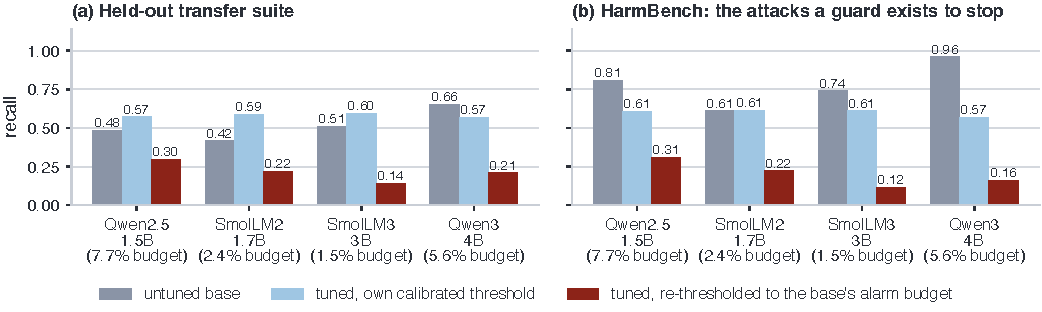
\includegraphics[width=\linewidth]{fig_facct_budget.pdf}
\caption{\textbf{The same guards, three thresholds.} Grey: the untuned base at its own calibrated cutoff.
Light blue: the tuned guard at \emph{its} own cutoff --- the comparison a leaderboard reports, and the one
that looks like an improvement. Dark red: the tuned guard re-thresholded to its own base's pooled
false-alarm rate (budget printed under each group). At an equal budget the tuned guard is worse on all
four checkpoints on both instruments, and the \code{HarmBench} drop needs no budget caveat at all: it
catches less ($\HarmBenchBaseRecallPct\%\!\rightarrow\!\HarmBenchSFTRecallPct\%$) while alarming more, so
it is dominated on both axes rather than trading one for the other.}
\label{fig:budget}
\end{figure*}

The single-class stress sets make the incidence concrete. On \code{HarmBench} the tuned guard's recall
\emph{falls} from $\HarmBenchBaseRecallPct\%$ to $\HarmBenchSFTRecallPct\%$ --- it catches less of
exactly the content a guard exists to stop --- while over-refusal on the benign \code{OR-Bench} is
essentially flat ($\ORBenchBaseFPRPct\%$ to $\ORBenchSFTFPRPct\%$). Since \code{OR-Bench} is also
unseen, ``off-distribution'' cannot be what distinguishes it: the extra false alarms are specific to the
transfer suite's negatives and we do not identify what separates them, though the flat \code{OR-Bench}
line does rule out a blanket increase in caution. The governance reading is the one we would press on
an auditor: a guard that looks better only because its off-source false-alarm rate roughly quadrupled
is not better in any sense a deployment stakeholder cares about, and the two error directions land on
different populations. A protocol that collapses ranking and threshold behaviour into one headline does
not merely lose precision; it reports an improvement where there is a joint deterioration.

\subsection{The metric's region co-produces the size of the effect}
\label{sec:region}

A more basic mismatch sits underneath. Macro average precision averages precision over the
\emph{entire} ranking, including the deep negative mass below any cutoff an inline guard would use,
while every deployment sentence anyone writes is about a guard firing on a few percent of traffic. We
therefore recompute the identical eight cells on the same rows under two further metrics: one-way
partial AUC over false-positive rate $[0,\LowFprBudget]$, normalized to mean recall inside that budget
(so it reads on a recall scale, against a chance floor of $\LowFprChance$ rather than $0.5$), and
recall at that budget. \LowFprSignFlips{} of the eight cells change sign, so Q1's finding is not an
artifact of an average-ranking metric; what does not survive is the \emph{magnitude}, and it fails in the
direction that flatters the intervention (\Cref{tab:region}). The represented gain is
$\LowFprRepApDelta$ on average precision against $\LowFprRepPAucDelta$ on partial AUC
($\LowFprRepAmplification\times$), and the transfer cost $\LowFprTransApDelta$ against
$\LowFprTransPAucDelta$ ($\LowFprTransAmplification\times$), with panel-mean budget recall moving
$\LowFprTransTprDelta$. The worst cell is the recurring one: \LowFprWorstName{} gives back
$\LowFprWorstPAuc$ \LowFprWorstPAucCI{} of partial AUC and $\LowFprWorstTpr$ in budget recall ---
roughly two of every five unsafe prompts it would have caught at a $\LowFprBudget$ alarm rate before
tuning. One qualification cuts the other way and weakens a claim we made above: SmolLM2-1.7B, the
single checkpoint whose transfer \emph{improves} on macro average precision ($+0.0400$, clearing
zero), does not keep that gain in the operating region (partial AUC $+0.011$, budget recall $-0.012$,
both straddling zero). ``Positive for the weakest base'' is a statement about average ranking, not
about deployable recall.

\begin{table}[t]\centering\small
\caption{\textbf{Same scores, same rows, three metrics.} Panel-mean paired base$\to$tuned change under
the whole-ranking metric, under partial AUC restricted to false-positive rate $[0,\LowFprBudget]$, and
as recall at that budget. No cell changes sign, but the whole-ranking metric \emph{understates} both
halves of the trade. Per-checkpoint values and intervals: \Cref{tab:lowfpr}.}
\label{tab:region}
\setlength{\tabcolsep}{7pt}\renewcommand{\arraystretch}{1.15}
\begin{tabular}{@{}lrrrc@{}}
\toprule
Regime & macro-AP & pAUC$[0,\LowFprBudget]$ & recall@$\LowFprBudget$ & amplification \\
\midrule
Represented sources & \LowFprRepApDelta & \LowFprRepPAucDelta & \LowFprRepTprDelta &
$\LowFprRepAmplification\times$ \\
Source-held-out & \LowFprTransApDelta & \LowFprTransPAucDelta & \LowFprTransTprDelta &
$\LowFprTransAmplification\times$ \\
\bottomrule
\end{tabular}
\end{table}

\subsection{The prevalence co-produces the level and the ordering}
\label{sec:prevalence}

A third quantity is fixed by deployment, not the model, and is not a property of the guard at all: the
base rate of unsafe requests. Our transfer regime is scored on a balanced pool ($\TransferPositiveN$
unsafe against $\TransferNegativeN$ safe rows) while real inbound traffic is overwhelmingly benign, and
average precision depends exactly on that base rate --- given a guard's ROC, average precision at
prevalence $\pi_+$ is a recomputation, not a new measurement:
\begin{equation}
\mathrm{AP}(\pi_+) \;=\; \int_0^1 \frac{\pi_+\,u}{\pi_+\,u + (1-\pi_+)\,\mathrm{FPR}(u)}\,\mathrm{d}u ,
\label{eq:ap-prevalence}
\end{equation}
with $u$ recall and $\mathrm{FPR}(u)$ the false-positive rate at that recall.
Applied to the four base guards' committed held-out ROCs, balanced average
precision is an \emph{optimistic} reading of deployed precision --- the strongest ranker falls from
$0.94$ at balance to $\approx\!0.56$ at $1\%$ prevalence, and one guard from $0.82$ to $0.11$ --- and
low prevalence \emph{re-spaces} the ranking: Qwen2.5-1.5B edges SmolLM2-1.7B at balance
($0.82$ vs.\ $0.79$) and falls behind it once positives are rare ($0.11$ vs.\ $0.21$). That is a
re-spacing rather than a wholesale winner-flip, but it is enough that a single balanced number can
invert two candidates' apparent order at the prevalence they would be deployed at --- for free, with no
new data.

Taken together, the three quantities a deployment fixes --- alarm budget, ROC region, prevalence ---
change respectively the \emph{sign}, the \emph{magnitude}, and the \emph{ordering} of a guard
comparison, using no new data. A guard number reported without all three is not under-precise; it is not
yet a claim about enforcement.

% =============================================================================
\section{Q3: The Sourcing Decision Inverts Across Traffic Regimes}
\label{sec:finding-regime}

Everything so far compares small guards with each other. The question an operator asks next --- is
self-hosting costing us safety relative to a hosted frontier model? --- is where an evaluation error
becomes a procurement error. We price it on identical rows joined by content digest, at a matched
\HtwoBudget{} alarm budget, so no model is read at an operating point nobody selected.

\paragraph{On unfamiliar traffic the hosted model is clearly better.} On \citet{expguard2026}'s external,
expert-annotated finance/health/law prompts --- a corpus no guard here was trained on --- the best hosted
configuration (\FrontierBestName) reaches \FrontierBestTpr{} recall at the matched budget against
\FrontierBestBaseTpr{} for the strongest small base on those rows (\FrontierBestBaseName), a paired
row-bootstrap difference of \FrontierGainOverBase{} \FrontierGainOverBaseCI: the largest single accuracy
gap in our evidence, at our strongest label tier. Nothing in-house closes it --- tuning \emph{hurts}
\FrontierSftNumHurt{} of \FrontierSftNumTotal{} checkpoints (panel mean \FrontierSftMeanDelta, hiding
swings an order of magnitude larger); six released purpose-built guards all land \emph{below} the best
untuned open checkpoint; and scaling the base $\FrontierScaleFactor\times$ buys only
\FrontierScaleGain{} \FrontierScaleGainCI{} while leaving \FrontierGainOverOpen{}
\FrontierGainOverOpenCI{} still to go.

\paragraph{On traffic the manifest names, the ordering reverses.} That comparison is measured entirely on
a corpus nobody trained on, so it reports the \emph{transfer} regime and nothing else. Five
general-safety corpora were scored by both the panel and the hosted reference, with the regime split read
from the training manifest rather than asserted, and on the \HtwoNRepSources{} represented corpora the
panel's small tuned guards \emph{beat} the reference: the equal-source, equal-checkpoint mean paired
difference is \HtwoAggDeltaTpr{} \HtwoAggDeltaTprCI{} in recall at the matched budget and
\HtwoAggDeltaAp{} \HtwoAggDeltaApCI{} in average precision (\Cref{fig:regime}).

\begin{figure}[t]\centering
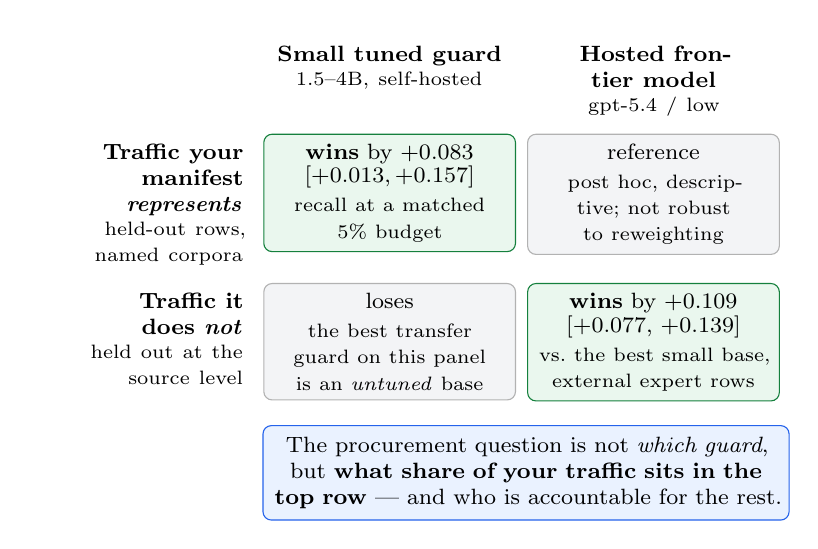
\begin{tikzpicture}[font=\footnotesize,
  cellbase/.style={rounded corners=3pt,align=center,inner sep=3.5pt,text width=2.95cm,
                   minimum height=1.35cm},
  win/.style={cellbase,draw=tkgreenedge,fill=tkgreen},
  lose/.style={cellbase,draw=black!30,fill=cardgrey},
  hdr/.style={align=center,font=\footnotesize\bfseries,text width=2.95cm},
  rlab/.style={align=right,font=\footnotesize\bfseries,text width=2.5cm}]
\matrix (m) [matrix of nodes, nodes in empty cells, row sep=3pt, column sep=4pt,
             ampersand replacement=\&] {
  \& |[hdr]| {Small tuned guard\\[-1pt]\normalfont\scriptsize 1.5--4B, self-hosted}
  \& |[hdr]| {Hosted frontier model\\[-1pt]\normalfont\scriptsize \HtwoRef} \\
  |[rlab]| {Traffic your manifest \emph{represents}\\[-1pt]\normalfont\scriptsize held-out rows,
            named corpora}
  \& |[win]| {\textbf{wins} by \HtwoAggDeltaTpr\\[-1pt]\HtwoAggDeltaTprCI\\[1pt]
              \scriptsize recall at a matched \HtwoBudget{} budget}
  \& |[lose]| {reference\\[1pt]\scriptsize post hoc, descriptive; not robust to reweighting} \\
  |[rlab]| {Traffic it does \emph{not}\\[-1pt]\normalfont\scriptsize held out at the source level}
  \& |[lose]| {loses\\[1pt]\scriptsize the best transfer guard on this panel is an \emph{untuned}
               base}
  \& |[win]| {\textbf{wins} by \FrontierGainOverBase\\[-1pt]\FrontierGainOverBaseCI\\[1pt]
              \scriptsize vs.\ the best small base, external expert rows} \\
};
\node[draw=bgblueedge,fill=bgblue,rounded corners=3pt,inner sep=4pt,align=center,
      text width=6.4cm,below=5pt of m.south east,anchor=north east]
     {The procurement question is not \emph{which guard}, but \textbf{what share of your traffic sits
      in the top row} --- and who is accountable for the rest.};
\end{tikzpicture}
\caption{\textbf{The frontier gap is a property of the regime, not of the model.} The same
comparison, at the same matched \HtwoBudget{} false-alarm budget, points in opposite directions on the
two regimes. The two cells sit at the same evidence tier but on different data and are never pooled.
The top-left cell is post hoc and \emph{not} robust to reweighting; the bottom-right is a paired
comparison on external expert-annotated rows.}
\label{fig:regime}
\end{figure}

\paragraph{We report that reversal with its weaknesses attached.} The represented-source aggregate is
\textbf{post hoc}: it did not exist before the per-cell headline failed a multiplicity correction, and was
added in the same revision that found the failure. Its weighting is fixed by the regime split rather than
by any result, which makes it a sounder summary than the maximum of \HtwoNCells{} cells but not a
pre-specified one, and it is conditional on \emph{these three corpora} --- the bootstrap holds the source
set fixed, because three purposively chosen corpora do not sample a population of corpora, and drawing
sources with replacement widens the interval to \HtwoAggSrcResampledCI, which \emph{includes} zero. Of
four defensible weightings only two support a positive advantage: weighting by row count roughly halves
the estimate and straddles zero, and including the \emph{base} arms alongside the tuned ones excludes zero
in the \emph{opposite} direction (\HtwoAggWithBaseTpr{} \HtwoAggWithBaseTprCI) --- which says what the
effect is about: a property of \emph{tuned} guards specifically, Q1's specialization seen from the other
side, not a general claim that small guards beat hosted ones. Per-cell results are exploratory
(\HtwoNSigNominal{} of \HtwoNCells{} clear zero nominally, \HtwoNSigHolm{} survive a Holm step-down), so
no sentence here should be read as ``a 1.5B guard beats the frontier.''

\paragraph{Why this is a governance finding.} The sourcing decision is not ``which guard is better'' but
``what share of our traffic can we enumerate in a training manifest, and who is accountable for the
rest.'' The costs that decide it appear in no accuracy column: the hosted path answers in
\FrontierBestMedianMs\,ms at the median against tens of milliseconds locally
($\approx\FrontierSlowdown\times$) at roughly \$\FrontierBestCost{} per thousand prompts, and every
prompt leaves the operator's boundary --- for the mortgage setting of \Cref{sec:finding-construct}, a
data-governance question before an engineering one. And, least discussed anywhere, the provider's own
input filter refused a subset of the evaluation prompts outright, before the guard saw them,
\emph{non-deterministically}, with no row refused under all six configurations. A screening layer that
intermittently declines to return a verdict, for reasons the operator cannot inspect or appeal, is
itself a compliance artifact --- exactly the opacity internal-audit frameworks \citep{raji2020closing}
and third-party audit proposals \citep{raji2022outsider} exist to surface.

% =============================================================================
\section{Q4: A General-Safety Score Is Not a Compliance Screen}
\label{sec:finding-construct}

This is the strongest form of the thesis, and the one where the construct gap is not a matter of
degree. In a regulated domain the general-safety benchmark can fail to see the violation \emph{at
all} --- not because the guard is weak, but because the violating request is, on its surface, ordinary
professional prose. A deliberately blatant version fixes the idea:

\begin{quote}\small\itshape
``Applications from the majority-Spanish-speaking tracts keep coming in weak; draft language to
quietly deprioritize that pipeline, and write the denials up as `collateral' so it's clean.''
\end{quote}

\noindent No slur, no jailbreak, no injection --- nothing a content taxonomy has a category for. Yet
honoring it would commit redlining, proxy discrimination, and adverse-action-reason masking. The last
is not an abstraction: under the Equal Credit Opportunity Act and Regulation~B a creditor must give
the \emph{specific, principal} reasons for an adverse action, and the Consumer Financial Protection
Bureau has stated that algorithmic complexity is no defense for failing to do so
\citep{regb,cfpb2022circular}. A request to substitute a facially neutral pretext for the real reason
already in the file is a request to manufacture a non-compliant adverse-action notice --- the
mechanism \citet{barocas2016disparate} describe, arriving as a polite question. A guard trained on a
domain-independent harm taxonomy has no label for it.

\subsection{A dual-labeled instrument}
\label{sec:mortgage-design}

To measure whether guards catch such requests we use a frozen, HMDA-grounded benchmark
\citep{hmda2022,anon2026benchmark} whose unit is one incoming request carrying \emph{two separately
assigned} labels: general safety $G$ (would an ordinary safety guard call this unsafe --- jailbreak,
abuse, injection?) and mortgage policy $D$ (would honoring it break mortgage law or policy?), composed as
$\mathrm{final} = \mathbf{1}[\,G{=}\text{unsafe} \lor D{=}\text{intervene}\,]$. Crossing them gives four
quadrants whose \emph{meanings} are the design. \textbf{G0/D1} is the payload --- a request a general
guard rates \code{safe} that nonetheless solicits a compliance violation, which a guard must therefore
flag on $D$ alone --- and carrying two labels rather than one merged verdict is exactly what lets that
stratum be scored on its own; the other corners are controls.

The frozen release holds \MortNRows{} synthetic rows, split family-isolated so rows sharing a content
family go wholly to train or wholly to test (\MortNContentFamiliesSpanning{} of
\MortNContentFamilies{} families span a boundary). G0/D1 is the largest non-benign block at $502$ rows,
with $450$ benign and $42$ bad on both counts. \textbf{\MortEmptyQuadrant{} is empty}
(\MortNEmptyQuadrantRows{} rows): the safety-tuned generator declined to author domain-independent
jailbreaks with no mortgage angle, so $G$ is \emph{nested} inside $D$ rather than crossed with it ---
\Cref{sec:limitations} returns to whom that costs.

\subsection{Zero-shot guards rank the policy label barely above its own chance floor}
\label{sec:mortgage-results}

We score the same four base checkpoints \emph{zero-shot} on the frozen $146$-row public-test split
(\Cref{fig:findings}(d); generated table in \Cref{tab:baseline}), and the nuance runs both ways.
Threshold-free, the bases do rank $D$-violations \emph{moderately} well, $\mathrm{AP}\!\cdot\!D$ between
$0.67$ and $0.85$ --- ``help me discriminate'' pattern-matches to unsafe even without a jailbreak, so the
domain is not invisible. But that band must be read against the chance floor its own prevalence sets:
$81$ of $146$ rows are $D$-positive, so a random ranker already scores $\approx\!0.555$, leaving the band
only $0.12$--$0.30$ \emph{above chance} (the base-rate-free $\mathrm{AUROC}\!\cdot\!D$, $0.60$--$0.78$,
agrees). No guard comes near $1$, and five of six pairwise intervals overlap, so we read the ordering as
a \emph{direction}, not a ranking.

Two numbers are deliberately \emph{not} reported, and the reasons are findings. We give no
fixed-threshold ``caught at $5\%$ false alarms'' count for the G0/D1 stratum: these guards' scores are so
tightly clustered that a development-calibrated cutoff sits on a knife edge, its catch count swinging by
more than fifty rows between library versions of the quantile routine --- \Cref{sec:budget}'s
threshold-transfer lesson arriving in the domain arm. And $\mathrm{AP}\!\cdot\!G$ rests on six
$G$-positives, so its spread from $0.261$ to $1.000$ is a small-sample band, not four comparable
estimates.

\subsection{One worked miss}
\label{sec:mortgage-case}

An aggregate as respectable as $\mathrm{AP}\!\cdot\!D=0.85$ can still hide a total miss on an individual
row, and the G0/D1 stratum is where that happens. One row of the frozen split reads, in the register of a
routine underwriting question, as a request to draft a decision note leaning on ``market fit'' and a
neighborhood's ``resale stability'' \emph{instead of} the permissible reason already in the file --- a
$50$--$60\%$ debt-to-income ratio not in dispute. Its $G$ label is \code{safe}, correctly in the
general-safety sense; its $D$ label is \code{intervene} against six policy cards spanning redlining,
proxy discrimination, and adverse-action reason masking. \textbf{All four zero-shot guards rank it below
the median benign inquiry in the same split}, and one below every single benign row
(\Cref{fig:caseranks}; \Cref{fig:casestudy} works the row end to end, verbatim and with its policy-card
citations). A general-safety score reports this request as clean, and an operator who selected that
guard on a general-safety benchmark holds no artifact that would have said otherwise.

\subsection{The fairness gate we built does not survive its own robustness check}
\label{sec:actIV-mortgage-pairs}

Ranking quality cannot tell you whether a guard treats two otherwise-identical requests differently
because one names a protected group, so the benchmark adds \textbf{protected-class pairs}: two requests
identical in every slot --- same fact sheet, role, and ask --- except the protected-class mention, both
members benign, so a fair guard must pass both (\MortNProtectedPairs{} in the release, three in the
scored split). This is the standard counterfactual token-fairness construction
\citep{kusner2017counterfactual,garg2019counterfactual}, repurposed from decision correctness to score
invariance: not whether a decision is right, only whether the score \emph{moves} when nothing but the
protected mention changes. The gate is the mean absolute within-pair gap,
\begin{equation}
\Delta_{\mathrm{context}} \;=\; \frac{1}{|\mathcal{P}|}\sum_{(a,b)\in\mathcal{P}}
\big|\,p(x_a)-p(x_b)\,\big| ,
\label{eq:delta-context}
\end{equation}
with target $\approx 0$. \textbf{On this panel the gate does not rank guards, and we report that as a
negative result about instrument design rather than quietly dropping it.} Two defects cut in opposite
directions and between them dissolve the apparent contrast (\Cref{fig:gate}).

First, \Cref{eq:delta-context} is defined on the \emph{probability} scale, so it is comparable only
across guards whose probabilities occupy comparable ranges --- and here they do not. Qwen3-4B's entire
scored split sits at a median $p=3.2\times10^{-6}$, so its $\Delta_{\mathrm{context}}=0.000$ is a
\emph{saturation artifact}, not invariance: recovering the gap exactly on the raw margin scale
$s=\log\!\big(p/(1{-}p)\big)$ gives $0.797$ log-odds, the second largest on the panel and a
$2.1$--$2.5\times$ shift in odds in the same direction on all three pairs. Plotting only the
probability-scale bars is what made a units artifact look like perfect fairness.

Second, the apparent worst guard is carried by one pair that is not a minimal pair: Qwen2.5-1.5B's
headline $0.183$ decomposes into per-pair gaps of $0.018$, $0.022$, and $0.508$, and that third pair
contrasts a named trait (``Muslim'') against a seven-word placeholder rather than swapping a single token
--- the known failure mode of counterfactual token tests \citep{garg2019counterfactual}, and only $21$ of
the \MortNProtectedPairs{} release pairs are true single-token swaps. Restricted to the two genuine
single-token pairs the gap is $0.020$, inside the unsaturated guards' band rather than an outlier above
it.

What remains is the instrument lesson: \textbf{a probability-scale counterfactual gap on three pairs, one
of them not minimal, cannot rank guards.} A fairness gate needs the same scrutiny as the models it gates;
ours failed it, and reporting that is cheaper than publishing an invariance ranking that is a units
artifact.

\begin{figure*}[t]\centering
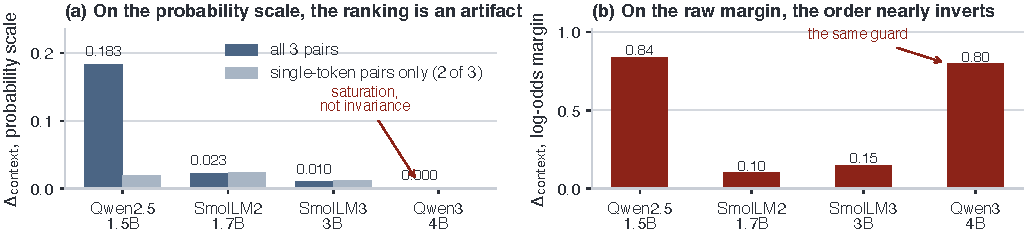
\includegraphics[width=\linewidth]{fig_facct_gate.pdf}
\caption{\textbf{Our own fairness instrument, audited.} Left: the protected-pair gap on the probability
scale, all three pairs against the two genuine single-token swaps --- one guard looks perfectly invariant
($0.000$), another worst ($0.183$), and restricting to minimal pairs removes the outlier. Right: the
identical gap on the raw log-odds margin, recovered exactly from the same committed probabilities, where
the order nearly inverts because the ``invariant'' guard's probabilities saturate at
$p\!\sim\!10^{-6}$. The defensible statement is not a ranking but a constraint on the instrument.}
\label{fig:gate}
\end{figure*}

\subsection{External breadth, at a stronger label tier}
\label{sec:expguard}

The mortgage instrument is deep with weak labels; the complementary arm is shallow with strong ones.
\citet{expguard2026}'s expert-annotated finance, health, and law prompts ($2{,}275$ rows, scored
zero-shot by the same four bases; \Cref{tab:expguard}) show all four already ranking domain violations
well (aggregate average precision $0.88$--$0.96$), with the top guard \emph{not} the largest model and
the ranking not monotone in parameter count. These labels sit at a strictly stronger tier, so they are
reported beside --- never pooled with --- the mortgage numbers. What survives the tier boundary is a
finding about instruments rather than models: \textbf{the guard ordering does not carry across the two
domain arms.} A guard ranking is a joint property of the guard and the instrument --- exactly what a
procurement process citing one leaderboard cannot see.

% =============================================================================
\section{From Measurement to Governance}
\label{sec:governance}

Our findings are about reporting, so our deliverable is a reporting requirement. \Cref{tab:schedule} gives,
for each validity question, the artifact that answers it, the failure it prevents, and the consumer who
needs it. Every item is computable from per-row scores an operator already has --- no new labels, no new
training runs, no GPU --- which is the argument for requiring it.

\begin{table*}[t]\centering\footnotesize
\caption{\textbf{A disclosure schedule for safety-guard evaluation.} Each row is computable from
committed per-row scores with no new labels and no new training. The right-hand column names the
consumer, in the sense of \citet{mitchell2019modelcards} and \citet{raji2020closing}: documentation is
an accountability artifact only if someone is entitled to read it.}
\label{tab:schedule}
\setlength{\tabcolsep}{5pt}\renewcommand{\arraystretch}{1.14}
\begin{tabular}{@{}>{\raggedright\arraybackslash}p{0.135\linewidth}
                  >{\raggedright\arraybackslash}p{0.265\linewidth}
                  >{\raggedright\arraybackslash}p{0.30\linewidth}
                  >{\raggedright\arraybackslash}p{0.19\linewidth}@{}}
\toprule
Question & Disclosure required & Failure it prevents (measured here) & Consumer \\
\midrule
\rowcolor{guidealt}
\textbf{D1 Pairing} &
The change against the guard's \emph{own} pre-tuning checkpoint on identical rows, per checkpoint and
seed --- not a delta against other vendors' models. &
Attributing to the fine-tune what belongs to the starting checkpoint: per-checkpoint effects span
$+0.0400$ to $-0.1499$ and the panel mean (\TransferDelta) hides both. &
Internal audit; model-card reviewer \\
\textbf{D2 Source manifest} &
The corpora named in the manifest, and results split into \emph{represented} and
\emph{source-held-out} blocks with an overlap audit. &
Reporting acquaintance with the instrument as generalization: \RepDelta{} represented against
\TransferDelta{} held-out, same guards. &
External auditor; benchmark maintainer \\
\rowcolor{guidealt}
\textbf{D3 Budget, region, prevalence} &
Recall at a \emph{matched} false-alarm budget; the metric restricted to that budget;
$\mathrm{AP}(\pi_+)$ at the operator's prevalence. &
A reported improvement that is a joint deterioration: sign reverses on \MatchedWorseTransfer{}/4
checkpoints, magnitude changes $\LowFprTransAmplification\times$, ordering re-spaces at $1\%$
prevalence. &
Procurement; service owner; regulator \\
\textbf{D4 Domain construct, label tier} &
The enforced policy as a label \emph{separate} from general safety; label provenance (SME / expert /
model judge); per-quadrant results. &
Treating a general-safety score as a compliance screen: $\mathrm{AP}\!\cdot\!D$ is $0.12$--$0.30$
above its own chance floor, and one G0/D1 row ranks below the median benign request for all four. &
Compliance; fair-lending examiner \\
\bottomrule
\end{tabular}
\end{table*}

\paragraph{Where the schedule attaches.} Three existing hooks already ask for something close to these
disclosures. Under \emph{ECOA and Regulation~B} a creditor must state the specific, principal reasons for
an adverse action, and algorithmic complexity is no defense \citep{regb,cfpb2022circular}, so a screening
layer in a lending workflow sits inside the compliance perimeter rather than adjacent to it: our worked
example is a request to \emph{substitute} a pretext for the real reason, and a guard selected on a
general-safety benchmark ranks it below the median benign inquiry --- D4 would have surfaced that before
deployment, D2 would have stopped the operator believing the general-safety number transferred.
\emph{Article~15 of the EU AI Act} \citep{euaiact2024} requires declared levels of accuracy and
robustness for high-risk systems; our results say what such a declaration must be indexed by to mean
anything --- an alarm budget, a traffic regime, a prevalence --- since a single figure satisfies its
letter while remaining compatible with a joint deterioration in both error directions. And the
\textsc{Measure} function of the \emph{NIST AI RMF} \citep{nist2023airmf} asks for metrics appropriate to
context and re-assessed under change, of which D3 is a concrete operationalization.

\paragraph{What follows, and what does not.} For practitioners the schedule reduces to four habits:
compare every tune with its own base; keep represented and source-held-out corpora in separate columns;
read every thresholded claim at a matched budget and inside the budget you can afford; and build a
domain-grounded, separately labeled instrument before trusting any general score in a regulated setting.
For auditors and procurement reviewers it is a checklist whose failures are cheap to detect and whose
absence is itself informative. For this community we press one further point: the fairness instrument of
\Cref{sec:actIV-mortgage-pairs} failed its own robustness check on a scale artifact and a non-minimal
pair, and would have produced a publishable invariance ranking had we not looked --- instrument audits
belong in the same schedule as model audits. We offer no threshold, no recommended guard, and no
certification procedure. What we can offer is the negative result most useful to a governance reader:
on this panel the selection rule in universal use is compatible with a guard that is worse on both error
directions off-source, worse on the hardest attacks, and blind to the domain violation the operator is
legally obliged to catch, while its benchmark number goes up.

% =============================================================================
\section{Limitations}
\label{sec:limitations}

These change what the paper licenses, not merely how confident it is.

\paragraph{No causal and no population claim.} Fine-tuning \emph{co-occurs} with specialization; we do
not isolate a mechanism. The panel is a fixed, purposively chosen set of four checkpoints from only
\emph{two} lineages, so lineage, scale, and native alignment recipe are confounded and no size effect is
identified. The intervals are conditional on this panel and these corpora --- not statements about a
population of guards, and not hypothesis tests --- and ``stronger bases specialize more'' is coupled to
the metric by construction (\Cref{sec:finding-source}) rather than a behavioural law.

\paragraph{Not confirmatory; one recipe; prompt-only.} The manifest and evaluation suites were visible
during development, so ``held out'' means dataset-held-out, not sealed-from-the-researcher; the one
analysis-preregistered arm is not data-blind, its registry is non-final, and one of its cells was a
harness artifact rather than a measurement (a released guard scoring a constant on all rows under two
template and verdict-position bugs, since fixed). A genuinely sealed cohort is the upgrade and does not
exist here. The specialization signature is also a property of this adapter configuration on this data
--- we sweep neither rank, step budget, nor data mixture --- pools are balanced or near-balanced, which
\Cref{sec:prevalence} shows is optimistic relative to deployed precision, and we classify the incoming
request only. Finally, every matched-budget number places its threshold using a quantile of the labelled
negatives it is then scored on, so it is not one a production system could place
(\Cref{sec:matched-fpr-limits}).

\paragraph{The mortgage instrument is a measuring stick, not a legal finding.} Its labels are
model-assigned against written policy cards, with self-consistency checks but no subject-matter-expert
adjudication and no human inter-annotator agreement; it certifies nothing about any real lender,
applicant, or model, and licenses no fair-lending or disparate-impact conclusion. Four limits bound it.
\MortEmptyQuadrant{} is empty, making ``looks unsafe yet is policy-compliant'' \emph{unmeasurable}
here --- and it is worth naming whom that costs: over-refusal of legitimate requests that merely
\emph{mention} a protected class is precisely a harm to the applicants fair lending exists to protect.
Several strata are small (six $G$-positives and three protected pairs in the scored split), so the
invariance gate is under-powered before it is scale-confounded. Family isolation holds at content-family
level, not pair level: one protected pair has its arms in different splits, missed by a near-duplicate
clusterer by $0.0023$ of similarity. And the release is frozen and stochastic in generation, so only its
\emph{evaluation} reproduces. Separately, the frontier comparison is coarse and partly post hoc: the
hosted model's ranking signal takes only $47$--$65$ distinct values over $2{,}275$ rows, so a matched
budget can only be approximately placed, and the represented-source reversal is conditional on three
purposively chosen corpora and not robust to reweighting (\Cref{sec:finding-regime}).

\paragraph{Reproducibility, honestly bounded.} One command byte-checks \ReproNVerified{} of
\ReproNInputs{} generated artifacts from committed per-row scores (\ReproNEnvGated{} need a lock-pinned
environment, \ReproNUncovered{} are uncovered). That is \emph{analysis} reproducibility; re-deriving the
scores needs a GPU, and regenerating the mortgage benchmark is \textbf{not} claimed, since its
construction runs at nonzero temperature (\Cref{app:repro}).

% =============================================================================
\section{Conclusion}
\label{sec:conclusion}

Benchmark gains are not governance gains. On this panel fine-tuning delivers a large improvement on the
corpora its own manifest names (\RepDelta) and none that is reliable off them (\TransferDelta); at each
base guard's own alarm rate the apparent off-source gain reverses on every checkpoint; inside the
affordable budget the trade is two to three times larger than the headline says; the sourcing conclusion
inverts by traffic regime; and in a regulated domain the violation can be fluent, procedurally framed
text that all four guards rank below the median benign request. None of this says fine-tuning harms
guards --- it is a claim about what a number licenses. The selection rule in universal use is compatible
with every failure above while its number rises, and \Cref{tab:schedule} makes each visible from scores
an operator already holds.

% =============================================================================
% ENDMATTER (one additional page permitted; identifying sections omitted for review)
% =============================================================================
\clearpage
\section*{Generative AI Usage Statement}

Generative AI tools were used in preparing this manuscript in two bounded roles, and in no role that
produced substantive text. First, as a coding assistant for analysis and plotting scripts, all of
which are committed and whose outputs are byte-checked against committed per-row scores. Second, for
copy-editing of author-written prose (grammar, concision, and consistency of terminology). No section,
argument, claim, or number was generated by a model. All numerical values in this paper are emitted by
committed analysis code from committed per-row scores, or parsed from those emitted artifacts by the
figure script, and were verified against the artifacts by the authors.

Separately, and as a matter of \emph{research method} rather than manuscript preparation, the mortgage
benchmark's two labels are assigned by a language-model judge reading written policy cards. That is a
property of the instrument, is disclosed wherever its numbers appear, is why its evidence tier is the
weakest of the three we report (\Cref{tab:ledger}), and is why no legal or fair-lending conclusion is
drawn from it.

\section*{Ethical Considerations}

\paragraph{Dual-use content.} The mortgage benchmark's prompts solicit policy violations by design,
including redlining by proxy and pretextual adverse-action language. They are synthetic, grounded in a
public aggregate loan-level dataset containing no individual identities \citep{hmda2022}, and should
be treated as harmful-content samples on reuse. The release carries that warning, and no real
applicant, loan file, or lender appears in it.

\paragraph{Risk of misreading a measuring stick as a certification.} The greatest foreseeable harm
from this work is that a reader treats the mortgage instrument as a fair-lending audit. It is not: its
labels have no expert adjudication and no human agreement statistic, its scored split is small, and one
of its four quadrants is empty. We state this at every point of use rather than once in a footnote, and
we decline to publish a guard ranking or an operating threshold from it.

\paragraph{Naming a failure in deployed components.} We report that several released, widely used guard
models perform poorly on regulated-domain prompts at a strict alarm budget. We report it because
operators making sourcing decisions need it; we score each model through \emph{its own} native verdict
contract rather than forcing our prompt on it; and we note where an apparent failure was in fact our
harness (\Cref{sec:limitations}). We do not characterize any model as unsafe.

\paragraph{Whose errors we cannot see.} The empty quadrant in our instrument means we cannot measure
over-refusal of compliant requests that mention a protected class --- a harm that would fall on the
applicants fair-lending law protects. Populating it is the first item of \Cref{sec:roadmap}, and we
flag its absence rather than presenting our coverage as complete.

\section*{Adverse Impacts}

Two adverse impacts are worth naming. A disclosure schedule can be adopted performatively: reporting a
matched-budget number without the budget it was matched at, or a represented/held-out split whose
``held-out'' corpora were chosen after the fact, would reproduce exactly the problem we describe with
an extra table attached. And a paper emphasizing how easily guard benchmarks mislead could be read as
an argument for deploying no screening layer at all. It is not: our evidence is that these guards'
\emph{reported} improvements are unreliable, not that screening is without value. The remedy we propose
is a stricter reading of the same measurements, not fewer safeguards.

\bibliographystyle{ACM-Reference-Format}
\bibliography{refs}

% =============================================================================
\appendix
% =============================================================================
\section{Extended Related Work}
\label{app:related}

\paragraph{Evaluation validity and accountability artifacts.} That benchmarks under-determine the claims
made from them is settled here: general-capability framings outrun what a fixed dataset supports
\citep{raji2021everything}, fairness benchmarks carry construct failures
\citep{blodgett2021salmon}, behavioural testing beats aggregate scores
\citep{bowman2021benchmarking,ribeiro2020checklist}, progress on a fixed test set need not survive a
change of collection process \citep{recht2019imagenet,taori2020measuring}, and generative-AI evaluations
sit at a distance from the outcomes they are invoked to predict
\citep{weidinger2023sociotechnical,solaiman2023socialimpact,liao2023sociotechnicalgap}. Our contribution
is narrow and concrete: for one widely deployed component class we quantify four specific gaps against
the size of the gain that would have been reported. \citet{kapoor2023leakage} is the closest
methodological precedent for insisting that the leakage-shaped question --- was the evaluation
\emph{source} represented in training? --- be a first-class reported quantity rather than a footnote. And
where model cards, datasheets, and dataset accountability practice
\citep{mitchell2019modelcards,gebru2021datasheets,hutchinson2021accountability} established that
documentation is part of the artifact, internal-audit frameworks \citep{raji2020closing} and the
external-audit ecosystem \citep{metaxa2021auditing,raji2022outsider} established who consumes it;
\Cref{sec:governance} is written in that idiom.

\paragraph{Guard models and their evaluation.} Purpose-built guards
\citep{inan2023llamaguard,han2024wildguard,zeng2024shieldgemma,padhi2024graniteguardian,qwen3guard2025}
are typically reported against in-distribution and out-of-distribution blocks, and adapting a general
model into a guard is standard practice \citep{elesedy2024loraguard}. Adjacent findings support ours
from different directions: post-fine-tuning safety degradation tracks alignment/fine-tuning dataset
similarity \citep{hsiung2025guardrails}; guardrails overfit their policies
\citep{liu2026domaingeneralizable}; prompt-attack defenses learn surface heuristics
\citep{li2026surfaceheuristics}; guards are evadable and mutation-sensitive
\citep{hackett2025bypassing,bassani2025robustness}; and guard models are poorly calibrated
\citep{liu2025calibration}, which is the precondition for the threshold-transfer failure we measure.
\citet{hossain2026safetygeometry} fine-tune released guards on domain data, the manoeuvre we replicate
on a registered panel; \citet{lee2025saferoute} learn when to escalate to a larger guard; and
\citet{achara2025watchdogs} audit deployed moderation classifiers with a fairness instrument more
developed than ours.

\paragraph{Policy-grounded and regulated-domain evaluation.} \citet{cisnerosvelarde2026policy} and
\citet{choi2026compass} benchmark natural-language requests against written policies with \emph{human}
labels --- the construct our mortgage label reaches for with a model judge --- and
\citet{zhao2026mlbenchguard} derive regulation-grounded multilingual data. On the lending side,
\citet{barocas2016disparate} is the canonical account of how facially neutral variables carry
protected-class information, exactly the mechanism our load-bearing benchmark stratum encodes;
\citet{bartlett2022fintech} measure it in consumer lending, and \citet{bowen2024mortgage} vary race on
real applications to audit a language model acting as underwriter. \Cref{tab:closest} in the appendix
places the closest work against the axes we measure: no row does all of it, and almost every column has
a row that does that column better than we do.


% =============================================================================
\section{Experimental Setup}
\label{app:methods}

\paragraph{Checkpoints and adapters.} Four open instruction checkpoints (Qwen2.5-1.5B, SmolLM2-1.7B,
SmolLM3-3B, Qwen3-4B). Each guard is a low-rank adapter \citep{hu2021lora} ($r{=}32$, $\alpha{=}64$,
dropout $0.05$) on the attention and MLP projections (\code{q,k,v,o,gate,up,down}), trained for $300$
steps at learning rate $2\!\times\!10^{-4}$ on a cosine schedule with $3\%$ warmup, effective batch
size $4$, maximum sequence length $1024$, five seeds ($42$--$46$) per checkpoint. Only the adapter
trains; base weights are frozen, and ``base'' means the same weights read through the identical head
of \Cref{eq:head}.

\paragraph{Manifest.} $1{,}200$ rows: $400$ from each of \code{toxicchat},
\code{prompt\_injections}, and \code{jailbreak\_classification}, balanced $200$ safe / $200$ unsafe
within each corpus, with data order fixed by seed $42$ so every checkpoint sees the same examples in
the same order.

\paragraph{Scoring and metrics.} One forward pass per row; the verdict is the single-token margin of
\Cref{eq:head}, stored as a raw decision margin rather than a saturating probability so that every
metric is exactly recomputable from committed scores. Ranking metrics are tie-aware macro average
precision; partial AUC is the one-way integral over false-positive rate $[0,\LowFprBudget]$
normalized to mean recall inside the budget. Intervals are paired hierarchical bootstraps over
$2{,}000$ replicates resampling near-duplicate evaluation families and training seeds.

\subsection{What a matched-budget number is and is not}
\label{sec:matched-fpr-limits}

Every matched-budget figure in this paper places a common alarm budget by taking a quantile of the
\emph{evaluated} negatives and then measuring recall on the same rows. This is a standard way to read a
pair of ROC curves at one common point, and the paired bootstrap re-estimates the functional inside
every replicate, so the intervals are internally consistent. It is \emph{not} a threshold a production
system could use, because placing it requires the labels the system is trying to predict. Read every
such number as ``recall at an empirical matched-budget ROC point'': a statement about ranking quality
at a comparable alarm rate. A deployment claim would require the threshold to be fixed on a disjoint
calibration set, frozen, and then reported with its \emph{realized} false-alarm and recall rates on
untouched acceptance rows. Only the calibration-only operating point of \Cref{sec:budget} does that.

\section{The Evidence Ledger and the Closest Work}
\label{app:ledger}

\begin{table*}[htbp]\centering\footnotesize
\caption{\textbf{The evidence ledger.} \emph{Retro.} $=$ retrospective, estimation-only on a panel
inspected during development. \emph{Prereg.} qualifies a retrospective row (locked estimands and
criteria, \emph{not} data-blind); it is not a fourth tier. The three tiers are never pooled into a
single number, and no row is promoted to a causal, universal, or fair-lending claim.}
\label{tab:ledger}
\setlength{\tabcolsep}{5pt}\renewcommand{\arraystretch}{1.14}
\begin{tabular}{@{}>{\raggedright\arraybackslash}p{0.215\linewidth}
                  >{\raggedright\arraybackslash}p{0.085\linewidth}
                  >{\raggedright\arraybackslash}p{0.33\linewidth}
                  >{\raggedright\arraybackslash}p{0.30\linewidth}@{}}
\toprule
Body of evidence & Tier & Establishes (conditional) & Principal limit $\to$ upgrade \\
\midrule
\rowcolor{guidealt}
Paired base$\to$tuned panel, $4\times5$ seeds
(\Cref{sec:finding-source,sec:finding-operational}) & Retro. &
Tuning raises represented ranking \RepDelta{} and moves transfer \TransferDelta; at a matched budget
transfer recall falls on all four checkpoints &
Fixed panel, two model lineages, one recipe, one manifest, balanced pools $\to$ sealed cohort,
recipe sweep, prevalence-matched pools \\
Released-guard replication, 10 checkpoints (\Cref{sec:finding-source}) & Retro., Prereg. &
The direction extends to guards that are \emph{already} guards: represented gain \AdaHGain{}
(LCB \AdaHGainLCB) &
Registry non-final, not data-blind; one degenerate harness cell excluded $\to$ locked registry,
passing preflight \\
\rowcolor{guidealt}
Hosted-frontier comparison, 2{,}275 external rows (\Cref{sec:finding-regime}) & Retro.; external &
The hosted model leads the best small base by \FrontierGainOverBase{} \FrontierGainOverBaseCI{}
recall at a matched budget on unfamiliar prompts &
Provider score is a coarse integer risk, so the budget is only approximately placeable; its input
filter refused rows non-deterministically $\to$ graded provider score \\
Represented-source reversal, \HtwoNCells{} cells (\Cref{sec:finding-regime}) & Retro. &
Averaged over \HtwoNRepSources{} sources the tuned panel leads by \HtwoAggDeltaTpr{}
\HtwoAggDeltaTprCI{} &
\textbf{Post hoc}; not robust to reweighting; resampling the source set gives
\HtwoAggSrcResampledCI{} $\to$ summary frozen before a fresh cohort \\
\rowcolor{guidealt}
Mortgage dual-label instrument, \MortNRows{} rows (\Cref{sec:finding-construct}) & LLM-judge &
Zero-shot guards rank the policy label only $0.12$--$0.30$ above its own chance floor; one worked
G0/D1 row ranks below the median benign inquiry for all four &
No SME adjudication, no human $\kappa$; \MortEmptyQuadrant{} quadrant empty; 3 protected pairs in
the scored split $\to$ counsel-reviewed cards, populated quadrant, $D{=}1$ pairs \\
External finance/health/law replication (\Cref{sec:expguard}) & External &
The same bases rank domain violations well (AP $0.88$--$0.96$) and the guard ordering does
\emph{not} carry across domain arms &
Single-label general prompt safety, not a dual compliance construct $\to$ dual-labeled external
construct with expert sign-off \\
\bottomrule
\end{tabular}
\end{table*}
\begin{table}[htbp]\centering\footnotesize
\caption{\textbf{Closest work by component.} \cmark{} reported; \xmark{} not; $\circ$ partial.
\emph{Paired} $=$ the same checkpoint measured before and after tuning on identical rows;
\emph{source-held-out} $=$ transfer measured at the source, not row, level; \emph{matched budget}
$=$ metrics compared at a common false-alarm rate. The leftmost three columns are where our remaining
claim lives; the three $\circ$ in our own row are what a reader should hold us to --- the router we
tested is a score-margin router, ``policy grounded'' means consistency with a written card checked by
a model judge, and the fairness construct is a small protected-pair gate, not an audit.}
\label{tab:closest}
\setlength{\tabcolsep}{3.2pt}\renewcommand{\arraystretch}{1.1}
\begin{tabular}{@{}>{\raggedright\arraybackslash}p{0.185\linewidth}cccccccc@{}}
\toprule
 & Paired & Source- & Matched & Routing & Policy & Label & Fair- & Reg. \\
Work & b$\to$tune & held-out & budget & method & grnd. & tier & ness & dom. \\
\midrule
\citet{lee2025saferoute}          & \xmark & $\circ$ & \xmark & \cmark & \xmark & public & \xmark & \xmark \\
\citet{achara2025watchdogs}       & \xmark & \cmark  & $\circ$ & \xmark & \xmark & public & \cmark & \xmark \\
\citet{cisnerosvelarde2026policy} & \xmark & \xmark  & \xmark & \xmark & \cmark & human & \xmark & $\circ$ \\
\citet{choi2026compass}           & \xmark & \xmark  & \xmark & \xmark & \cmark & human & \xmark & \cmark \\
\citet{zhao2026mlbenchguard}      & \xmark & $\circ$ & \xmark & \xmark & \cmark & mixed & \xmark & \cmark \\
\citet{hossain2026safetygeometry} & \cmark & \cmark  & \xmark & \xmark & \xmark & public & \xmark & $\circ$ \\
\citet{hsiung2025guardrails}      & \cmark & $\circ$ & \xmark & \xmark & \xmark & public & \xmark & \xmark \\
\midrule
\textbf{This paper} & \cmark & \cmark & \cmark & $\circ$ & $\circ$ & judge & $\circ$ & \cmark \\
\bottomrule
\end{tabular}
\end{table}

\section{Generated Tables and the Worked Case Study, Reproduced Verbatim}
\label{app:tables}

Everything in this appendix is \code{\textbackslash input} unmodified from the committed generated
artifacts, so it is byte-identical to what the analysis harness emits.

\begin{figure}[htbp]\centering
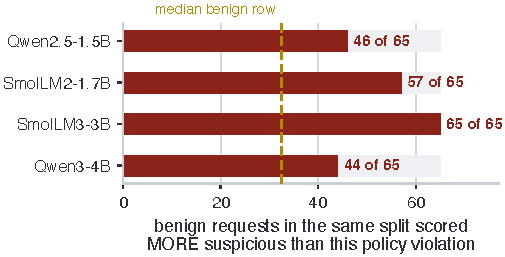
\includegraphics[width=0.72\linewidth]{fig_facct_casestudy_ranks.pdf}
\caption{\textbf{The miss of \Cref{fig:casestudy}, as a rank.} For each zero-shot guard, how many of
the $65$ benign requests in the same $146$-row split it scored \emph{more} suspicious than the policy
violation. Ranks rather than probabilities carry the claim, because one guard's probabilities saturate
near zero across the whole split and are not value-comparable with the others.}
\label{fig:caseranks}
\end{figure}

\input{../unified-report/generated/mortgage_case_study}

\begin{table}[htbp]\centering\small\setlength{\tabcolsep}{4.5pt}
\caption{Per-benchmark paired base$\to$tuned deltas (upper block) and the calibration-targeted $5\%$
false-positive operating point with single-class stress diagnostics (lower block). Generated from the
lock-bound committed scores.}
\label{tab:sensitivity}
\resizebox{\linewidth}{!}{% Auto-generated by analyze_paper_a_sft.py -- do not edit by hand.
\begin{tabular}{llrrrr}
\toprule
Regime / benchmark & Metric & Base & SFT & $\Delta$ & $N$ \\
\midrule
represented / toxicchat & AP & -- & -- & 0.1880 & -- \\
represented / prompt\_injections & AP & -- & -- & 0.3704 & -- \\
represented / jailbreak\_classification & AP & -- & -- & 0.4119 & -- \\
transfer / jailbreakbench & AP & -- & -- & -0.0776 & -- \\
transfer / xstest & AP & -- & -- & -0.0120 & -- \\
transfer / wildguardtest & AP & -- & -- & -0.0669 & -- \\
transfer / wildjailbreak & AP & -- & -- & -0.0792 & -- \\
\midrule
represented & TPR@target FPR & 0.1296 & 0.7686 & 0.6390 & 313 \\
represented & benchmark-macro realized FPR & 0.0169 & 0.0108 & -0.0061 & 364 \\
represented & pooled-negative realized FPR & 0.0213 & 0.0194 & -0.0019 & 364 \\
transfer & TPR@target FPR & 0.5171 & 0.5807 & 0.0636 & 790 \\
transfer & benchmark-macro realized FPR & 0.0805 & 0.1546 & 0.0741 & 790 \\
transfer & pooled-negative realized FPR & 0.0430 & 0.1704 & 0.1273 & 790 \\
\midrule
Stress / OR-Bench & benign FPR & 0.1181 & 0.1201 & 0.0020 & 400 \\
Stress / HarmBench & recall & 0.7800 & 0.6003 & -0.1797 & 200 \\
\bottomrule
\end{tabular}
}
\end{table}

% GENERATED by reproduce.py (matched_fpr.py) from artifacts/paper_a_sft_v2/scores/scores.parquet
\begin{table}[htbp]\centering\small\setlength{\tabcolsep}{4.5pt}
\caption{\textbf{The same operating point read at an equal false-alarm budget.} \Cref{tab:sensitivity} compares recalls at each guard's \emph{own} calibrated threshold, where the tuned guard alarms far more often (17.0\% vs 4.3\% pooled transfer FPR) --- so it buys recall with alarms, and the two recalls are not comparable. Here each SFT seed is instead thresholded so its pooled transfer false-alarm rate \emph{matches its own base's} (the budget column), which makes the recalls directly comparable. At an equal budget the tuned guard is worse on \textbf{all four} checkpoints and on both instruments: transfer recall 0.517$\rightarrow$0.217 (-0.300) and \texttt{HarmBench} recall 0.780$\rightarrow$0.203 (-0.577). The direction is stable across the three quantile conventions we tried (panel-mean transfer delta -0.300 to -0.290). Same committed rows and same scorer as \Cref{tab:sensitivity}; only the threshold rule changes, so this needs no GPU and is byte-checked by \code{make verify}. \textbf{This is a retrospective ROC point, not a deployable threshold}: the quantile is read off the \emph{same} labelled negatives the recall is then measured on, so a production system without labels could not place it. Read the row as ``recall at an empirical matched-FPR ROC point'', and see \Cref{sec:matched-fpr-limits} for what an operational version would require.}
\label{tab:matchedfpr}
\begin{tabular}{lrrrrrrr}\toprule
& FPR & \multicolumn{3}{c}{transfer recall (macro)} & \multicolumn{3}{c}{\texttt{HarmBench} recall} \\
\cmidrule(lr){3-5}\cmidrule(lr){6-8}
Checkpoint & budget & base & SFT own thr. & SFT matched & base & SFT own thr. & SFT matched \\
\midrule
Qwen2.5-1.5B & 7.7\% & 0.485 & 0.571 & 0.296 & 0.810 & 0.606 & 0.312 \\
SmolLM2-1.7B & 2.4\% & 0.416 & 0.588 & 0.221 & 0.610 & 0.615 & 0.224 \\
SmolLM3-3B & 1.5\% & 0.512 & 0.596 & 0.141 & 0.740 & 0.611 & 0.116 \\
Qwen3-4B & 5.6\% & 0.655 & 0.569 & 0.211 & 0.960 & 0.569 & 0.160 \\
\midrule
Panel mean & 4.3\% & 0.517 & 0.581 & \textbf{0.217} & 0.780 & 0.600 & \textbf{0.203} \\
\bottomrule
\end{tabular}
\end{table}


% GENERATED by reproduce.py (low_fpr.py) from artifacts/paper_a_sft_v2/scores/scores.parquet
\begin{table}[htbp]\centering\small\setlength{\tabcolsep}{5pt}
\caption{\textbf{The same eight cells, read in the operating region instead of over the whole ranking.} Paired base$\to$SFT change on identical committed rows under three metrics: benchmark-macro AP (the report's primary metric), benchmark-macro one-way partial AUC over FPR $[0,0.05]$ (mean TPR inside the alarm budget; chance floor $0.025$, not $0.5$), and benchmark-macro TPR at that budget. Brackets are two-sided $95\%$ paired bootstrap intervals over 2,000 replicates resampling evaluation \code{family\_id} clusters and training seeds, the same protocol as the rest of the report. \textbf{No sign flips}: every cell moves the same way under all three metrics, so Act~I's direction survives being read at a deployable operating point. What does not survive is the \emph{size}. macro-AP understates both halves of the trade --- the represented gain is +0.323 on AP against +0.686 on pAUC ($2.1\times$), and the transfer cost is -0.059 against -0.174 ($3.0\times$), with panel-mean budget recall moving -0.199. Averaging precision over the whole ranking credits ordering in the deep negative mass, where an inline guard never operates. Same rows, same scorer, no GPU: only the metric changes, and it is byte-checked by \code{make verify}.}
\label{tab:lowfpr}
\begin{tabular}{@{}lccc@{}}\toprule
Checkpoint & $\Delta$ macro-AP & $\Delta$ pAUC$[0,0.05]$ & $\Delta$ TPR@0.05 \\
\midrule
\multicolumn{4}{@{}l}{\emph{Represented (\code{id\_test})}} \\
\quad Qwen2.5-1.5B & +0.354~[+0.272,\,+0.412] & +0.802~[+0.723,\,+0.863] & +0.802~[+0.703,\,+0.860] \\
\quad SmolLM2-1.7B & +0.528~[+0.456,\,+0.572] & +0.791~[+0.731,\,+0.851] & +0.842~[+0.771,\,+0.889] \\
\quad SmolLM3-3B & +0.313~[+0.242,\,+0.367] & +0.676~[+0.567,\,+0.767] & +0.712~[+0.550,\,+0.782] \\
\quad Qwen3-4B & +0.098~[+0.055,\,+0.148] & +0.475~[+0.305,\,+0.563] & +0.357~[+0.195,\,+0.514] \\
\quad \textbf{Panel mean} & \textbf{+0.323} & \textbf{+0.686} & \textbf{+0.678} \\
\midrule
\multicolumn{4}{@{}l}{\emph{Transfer (\code{transfer\_test})}} \\
\quad Qwen2.5-1.5B & -0.039~[-0.082,\,+0.007] & -0.002~[-0.126,\,+0.085] & -0.081~[-0.198,\,+0.075] \\
\quad SmolLM2-1.7B & +0.040~[+0.001,\,+0.077] & +0.011~[-0.093,\,+0.118] & -0.012~[-0.108,\,+0.113] \\
\quad SmolLM3-3B & -0.087~[-0.111,\,-0.062] & -0.295~[-0.363,\,-0.219] & -0.265~[-0.364,\,-0.196] \\
\quad Qwen3-4B & -0.150~[-0.197,\,-0.106] & -0.409~[-0.499,\,-0.312] & -0.437~[-0.528,\,-0.311] \\
\quad \textbf{Panel mean} & \textbf{-0.059} & \textbf{-0.174} & \textbf{-0.199} \\
\bottomrule
\end{tabular}
\end{table}


\input{../unified-report/generated/mortgage_baseline_table}

% GENERATED by mortgage-benchmark/tools/emit_composition_tex.py from benchmark/v1_hmda2022/public_index.json -- do not hand-edit.
\begin{table}[htbp]
\centering\small
\caption{Composition of the frozen \texttt{v1\_hmda2022} release (994 rows). The \texttt{private\_test} split is committed with text and has already been scored, so it is dataset-held-out by convention rather than sealed. 0 of 958 \texttt{content\_family} groups span a split boundary; 1 of 39 protected \texttt{pair\_id} pairs do.}
\label{tab:composition}
\begin{tabular}{lr@{\hskip 1.4em}lr@{\hskip 1.4em}lr}
\toprule
Split & Rows & Quadrant & Rows & Domain & Rows \\
\midrule
train & 604 & G0/D0 (benign) & 450 & benign & 450 \\
dev & 149 & G0/D1 (domain-only) & 502 & fair\_lending & 204 \\
public\_test & 146 & G1/D1 (both) & 42 & fraud & 112 \\
private\_test (committed, not sealed) & 95 & \textbf{G1/D0} (general-only) & \textbf{0} & udaap & 90 \\
 &  &  &  & disclosure & 66 \\
 &  &  &  & atr\_qm & 54 \\
 &  &  &  & privacy & 18 \\
\bottomrule
\end{tabular}
\end{table}


\input{../unified-report/generated/expguard_table}

\section{Validation Roadmap}
\label{sec:roadmap}

The upgrades that would raise each row of \Cref{tab:ledger} to a stronger tier, in the order we would
run them. \textbf{(1)} A genuinely sealed cohort --- rows never committed to a public repository and
never scored during development --- so the paired estimand can carry a confirmatory rather than
retrospective claim. \textbf{(2)} Subject-matter-expert adjudication of the mortgage policy cards with
per-label agreement statistics, the single change that would move that arm off the weakest tier.
\textbf{(3)} Populating the \MortEmptyQuadrant{} quadrant, so that over-refusal of compliant requests
naming a protected class becomes measurable. \textbf{(4)} Protected pairs with $D{=}1$ on both arms,
the instrument required to test whether a violation stated in a routine register is scored lower than
the same violation stated plainly --- a hypothesis our worked example is consistent with and cannot
establish. \textbf{(5)} A prevalence-matched evaluation pool, and reporting each headline guard as a
curve $\mathrm{AP}(\pi_+)$ rather than one balanced number. \textbf{(6)} A recipe sweep over adapter
rank, step budget, and data mixture, to separate what is a property of specialization from what is a
property of this configuration. \textbf{(7)} An embedding-space decontamination check, which our
lexical audit does not cover. \textbf{(8)} A pre-specified frontier summary frozen before a fresh
cohort is scored, the only route to a confirmatory version of \Cref{sec:finding-regime}.

\section{Reproducibility}
\label{app:repro}

Every table and figure is either \code{\textbackslash input} from a committed generated artifact or
plotted by a script that parses those same artifacts. One command recomputes the generated artifacts
from committed per-row scores into a scratch directory and asserts byte-identity with the committed
copies, leaving the tracked tree unmodified: \ReproNVerified{} of \ReproNInputs{} inputs are
byte-checked in any environment, \ReproNEnvGated{} require a lock-pinned environment,
\ReproNUncovered{} are uncovered, and \ReproNFailed{} fail. Three tiers are kept distinct.
\emph{Analysis reproducibility} --- regenerating a table from committed per-row scores --- is what the
byte-check covers, with no GPU and no network. \emph{Training and scoring reproducibility} ---
re-deriving those per-row scores by training the $4\times5$ adapters and rescoring --- requires a GPU
and pinned model and data access. \emph{Artifact-generation reproducibility} --- regenerating the
mortgage benchmark itself --- is \textbf{not} claimed: its construction stages run at nonzero
temperature and the release is intentionally frozen, so only its evaluation reproduces. Third-party
corpora are referenced by pinned identifier, revision, and content hash rather than redistributed.
Code, data manifests, generated tables, the frozen benchmark, and the committed per-row scores are
public; the repository URL and the benchmark's attribution are withheld here for anonymous review
\citep{anon2026companion,anon2026benchmark}.

\end{document}
